\documentclass[12pt,a4paper]{article}

\usepackage{fontspec}
\usepackage{xeCJK}
\usepackage{graphicx}
\usepackage[normalem]{ulem}
\usepackage{geometry}
\usepackage{hyperref}

\geometry{a4paper,margin=2.5cm}

\setmainfont{TeX Gyre Termes}
\setCJKmainfont{Noto Serif CJK SC}

\newcommand{\ul}[1]{\underline{#1}}

\setlength{\parindent}{0pt}
\setlength{\parskip}{0.3em}

\begin{document}

\begin{center}
  {\LARGE\bfseries 《系统开发工具基础》实验报告}

  \vspace{1.2em}

  \renewcommand{\arraystretch}{1.6}
  \begin{tabular}{l@{\hspace{1em}}l@{\hspace{3em}}l@{\hspace{1em}}l}
    \textbf{姓名\hspace{2em}：} & \ul{夏昕} & \textbf{学号\hspace{2em}：} & \ul{25080012068} \\
    \textbf{专业\hspace{2em}：} & \ul{软件工程} & \textbf{任课教师：} & \ul{周小伟} \\
    \textbf{实验时间：} & \ul{2026/8/31} & \textbf{实验周次：} & \ul{第 2 周} \\
  \end{tabular}

  \vspace{1.2em}

  \textbf{GitHub仓库链接：}\url{https://github.com/ztmy1110/system-development-tools}

  \vspace{1em}

  {\Large\bfseries commit 记录}
\end{center}

\noindent\rule{\linewidth}{0.4pt}

\medskip

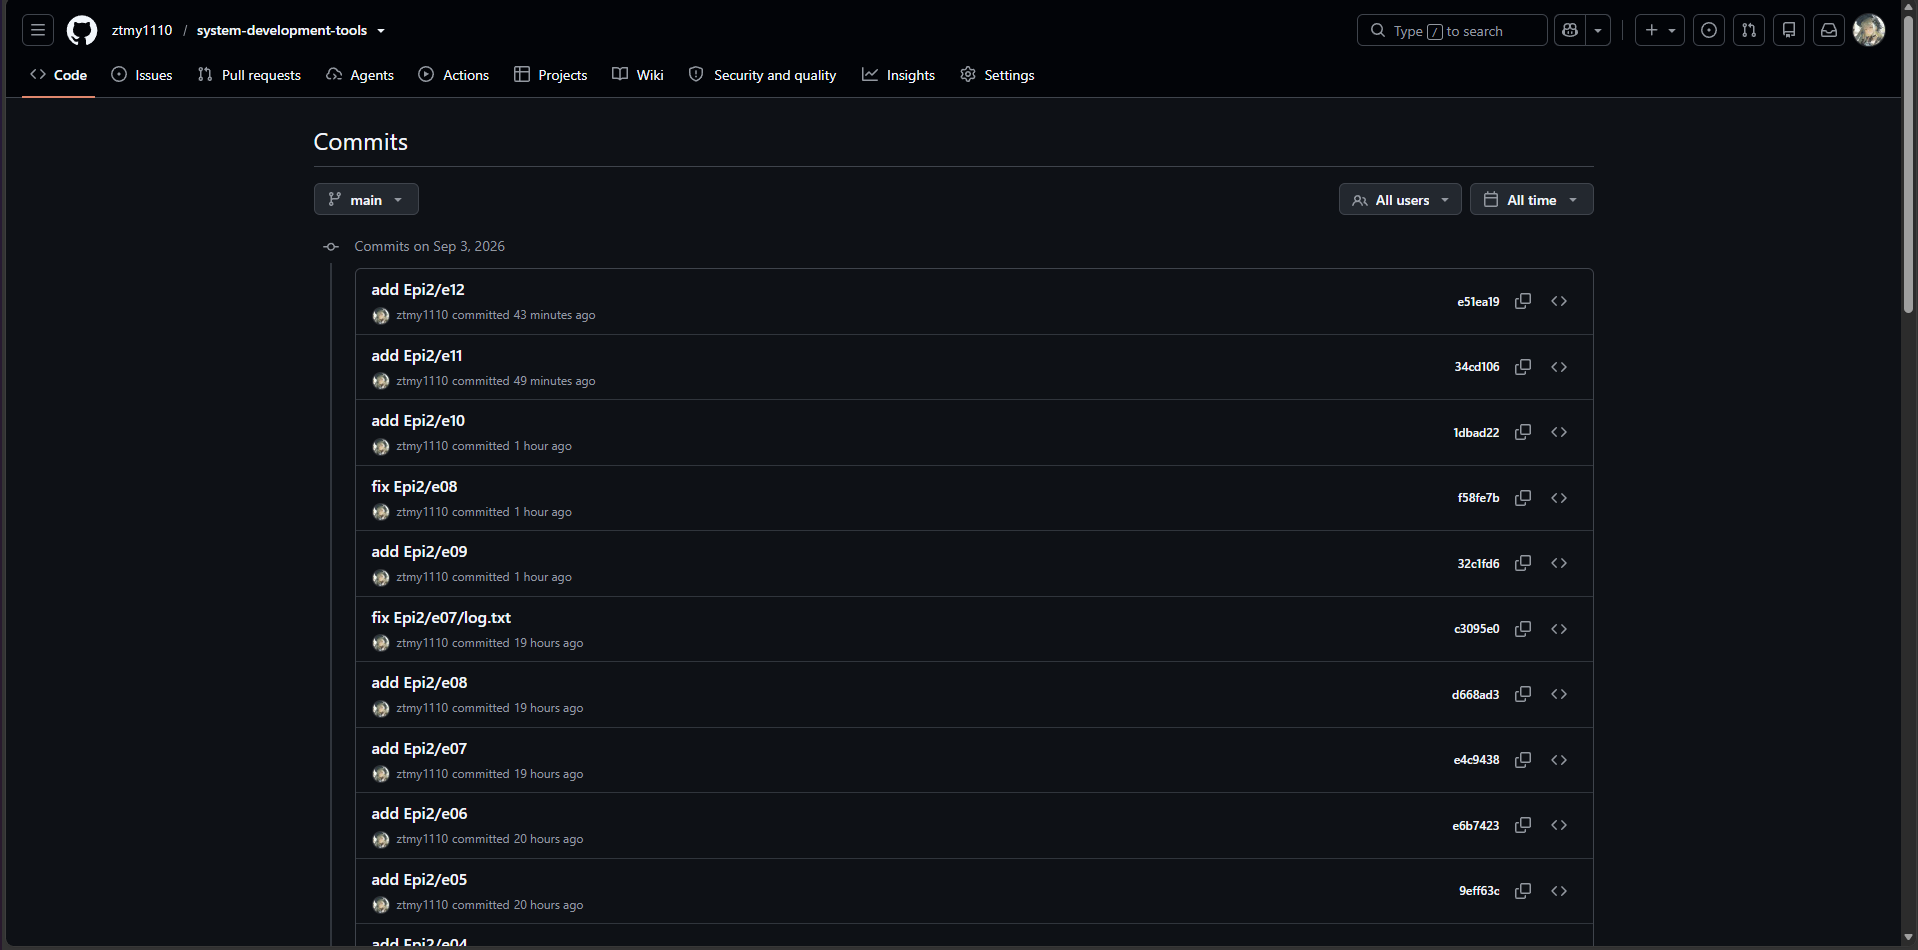
\includegraphics[width=6.65354in,height=3.8132in]{media/media/commit.png}

\textbf{课堂习题}

\vspace{1em}
\textbf{第5题：控制一个可清理的后台任务}

\vspace{0.6em}
\textbf{一、主题}

命令行环境：进程、信号与任务控制

\vspace{0.6em}
\textbf{二、题目要求}

1. 将给定的 worker.sh 脚本保存到 q05/，赋予脚本执行权限，在前台启动，并将标准输出和标准错误分别保存到 stdout.log 和 stderr.log。

2. 使用 Ctrl-Z 挂起任务，再使用 bg 让任务在后台继续运行，并使用 jobs 查看任务状态。

3. 使用 jobs -p 或等价方法获取任务 PID，不能手工抄写 PID，然后发送 SIGTERM，等待任务正常结束。禁止使用 kill -9。

4. 检查 cleanup.log，确认其中出现 CLEAN\_EXIT，同时确认后台任务已经退出。

\vspace{0.6em}
\textbf{三、源程序代码}

chmod +x worker.sh

./worker.sh > stdout.log 2> stderr.log

bg

jobs

jobs -p | xargs kill

jobs

\vspace{0.6em}
\textbf{四、程序运行结果}

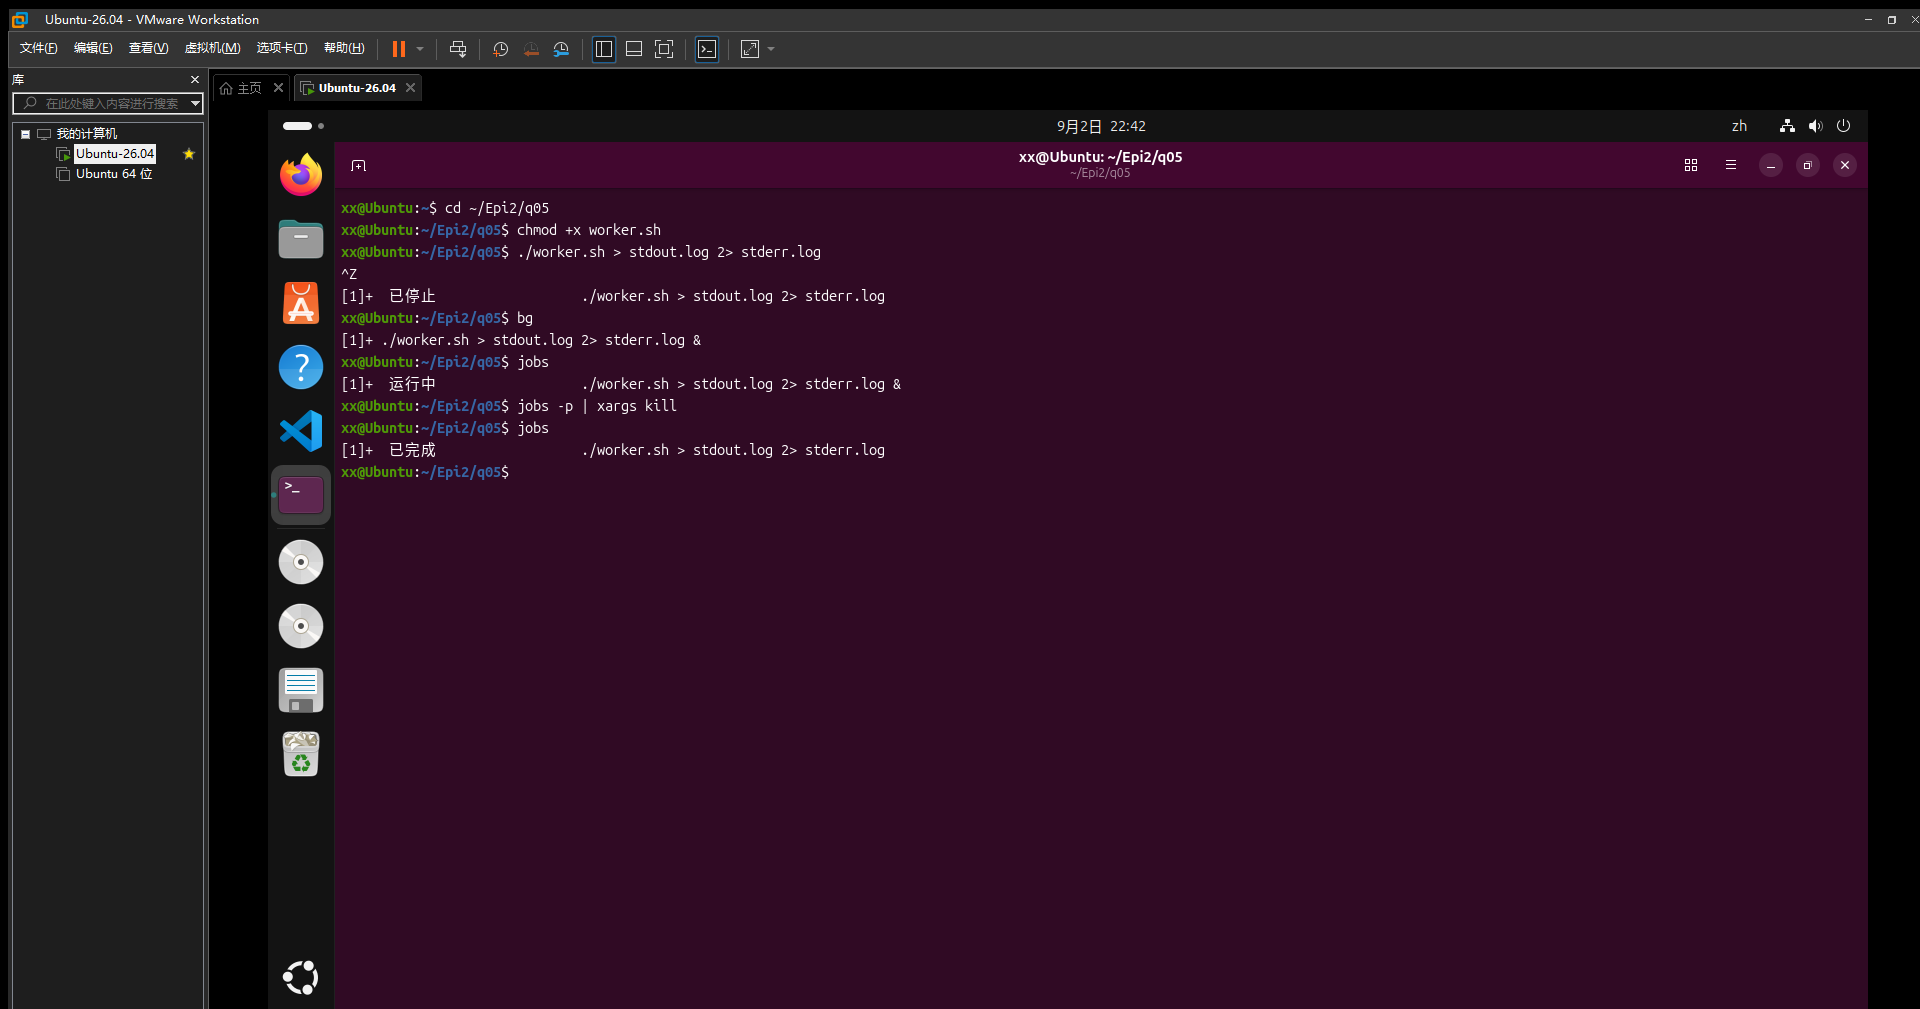
\includegraphics[width=6.65694in,height=3.95556in]{media/media/q05_1.png}

\vspace{0.6em}
\textbf{五、解题感悟}

1. 这次主要熟悉了前台任务和后台任务之间的切换，之前对 Ctrl-Z、bg 和 jobs 的作用不太清楚，实际操作后比较直观。

2. 通过 jobs -p 获取 PID 比手动找进程号方便，也能减少输错 PID 的情况。

3. 这道题让我知道了程序不一定要直接强制结束，通过信号让程序自己完成清理后退出会更加合理。

\vspace{1em}
\textbf{第6题：语义重构与本地开发反馈}

\vspace{0.6em}
\textbf{一、主题}

开发环境与工具

\vspace{0.6em}
\textbf{二、题目要求}

1. 在已经配置好 Python、pytest 和 ruff 的课程环境中打开 q06，并启用 Python 语言服务器。

2. 分别使用编辑器的跳转到定义和查找引用功能，查看 total\_price 的定义和使用位置。

3. 使用“重命名符号”功能，将 total\_price 修改为 calculate\_total，保证定义和所有引用同步修改。

4. 在 app.py 中临时加入未使用的 import os，使用 ruff 检查并发现问题，然后删除该无用导入。

5. 最后运行 ruff 和 pytest，保证代码检查和测试都通过。

\vspace{0.6em}
\textbf{三、源程序代码}

无

\vspace{0.6em}
\textbf{四、程序运行结果}

转到定义和查找引用：

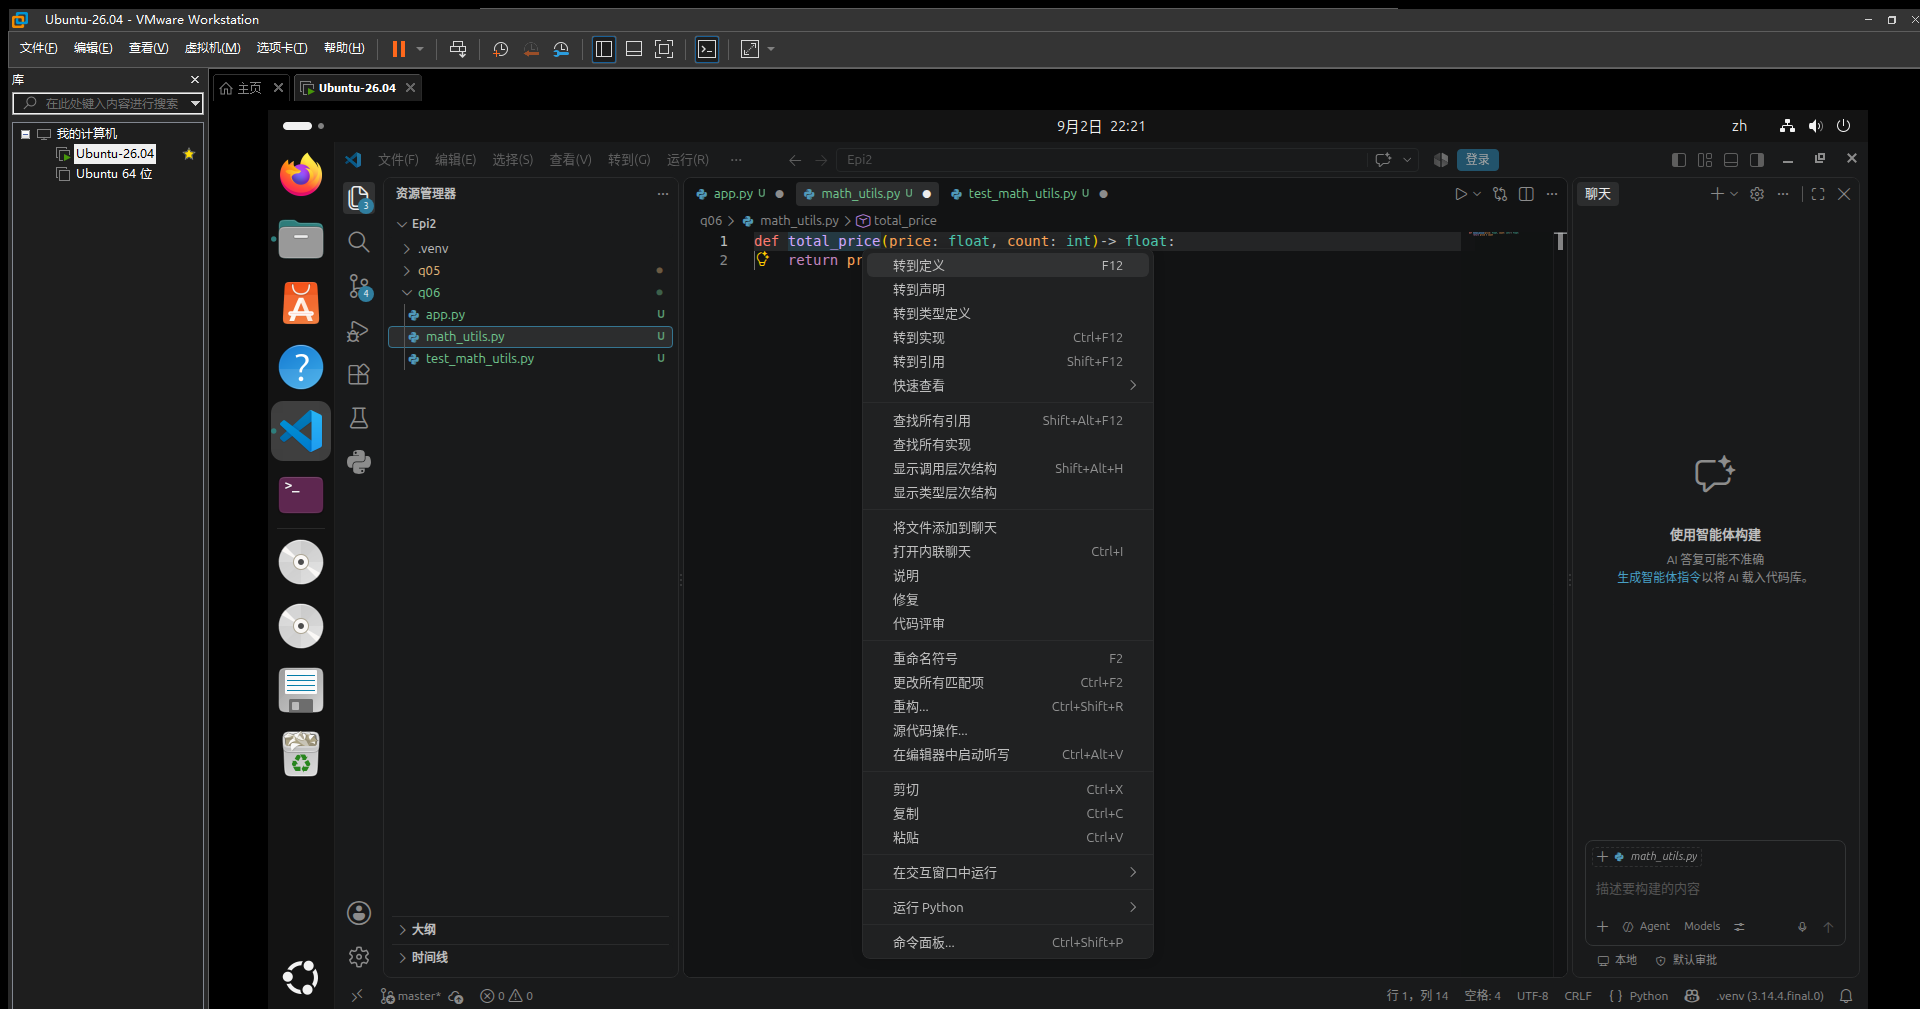
\includegraphics[width=6.65694in,height=3.95556in]{media/media/q06_1.png}

重命名符号：

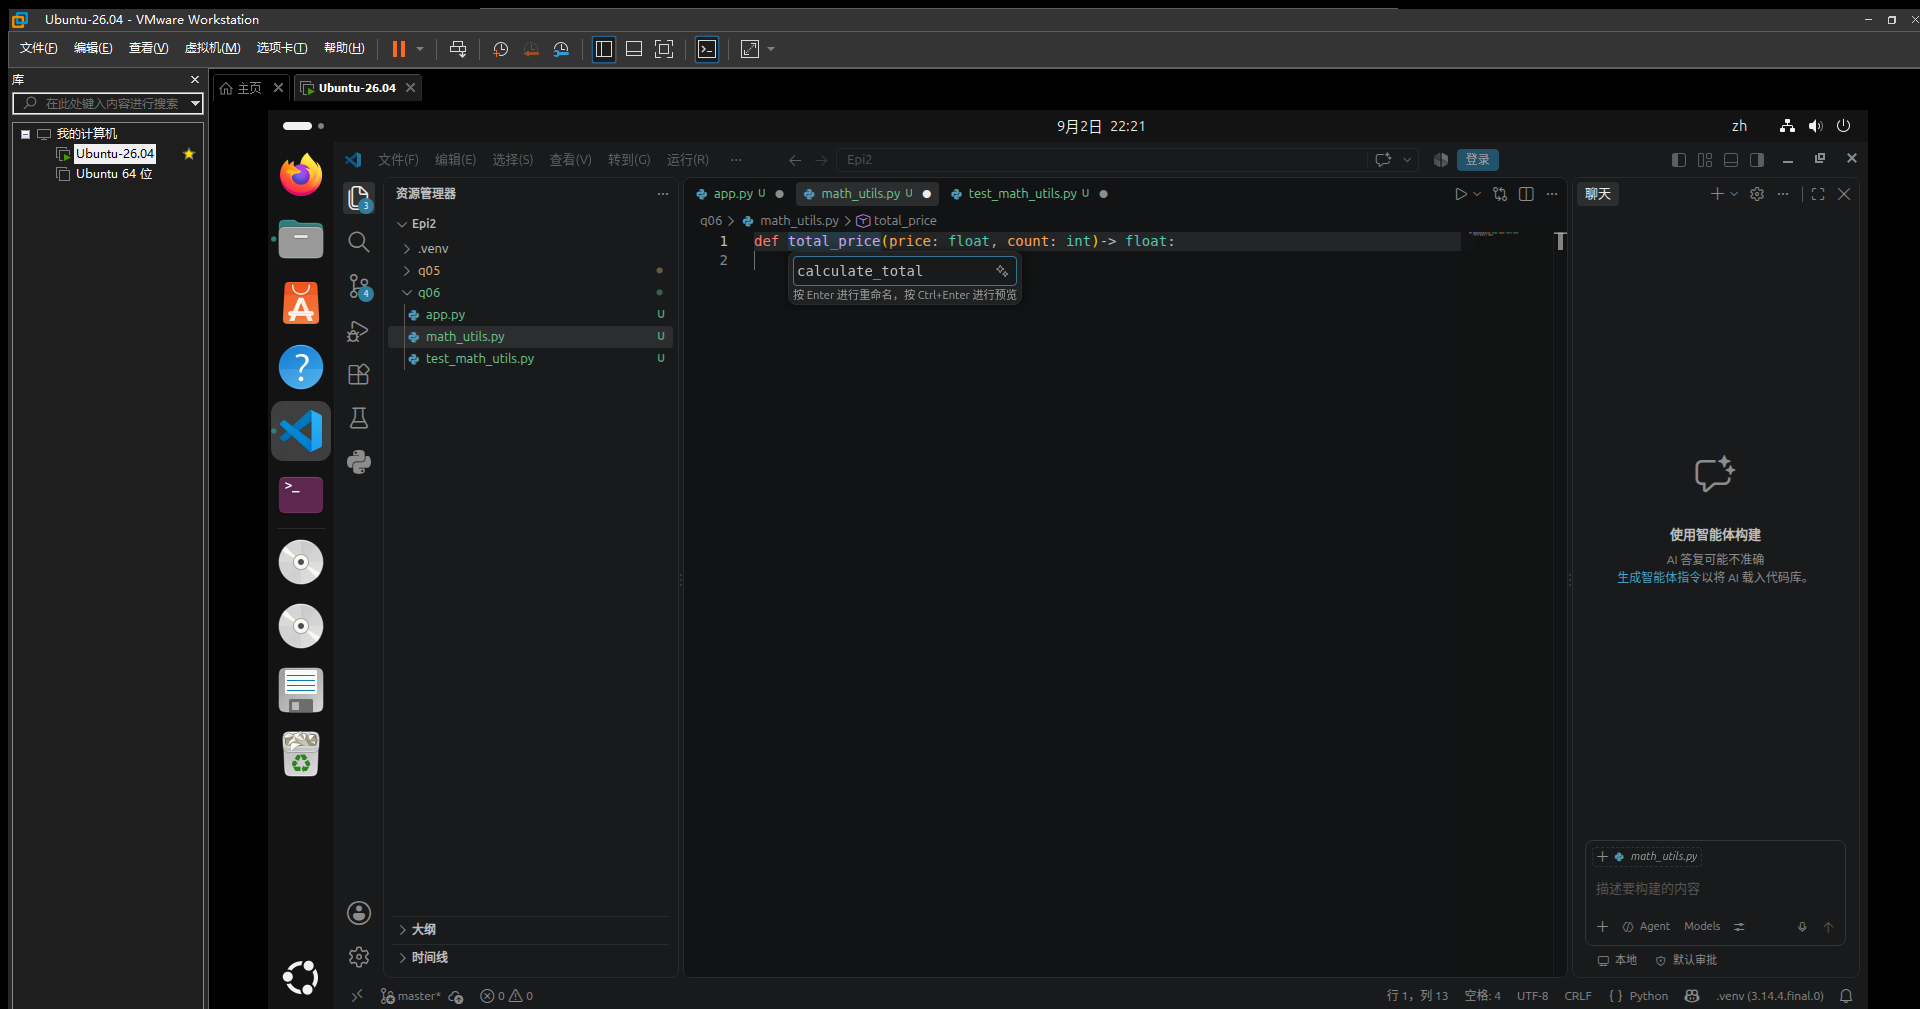
\includegraphics[width=6.65694in,height=3.95556in]{media/media/q06_2.png}

改错和pytest：

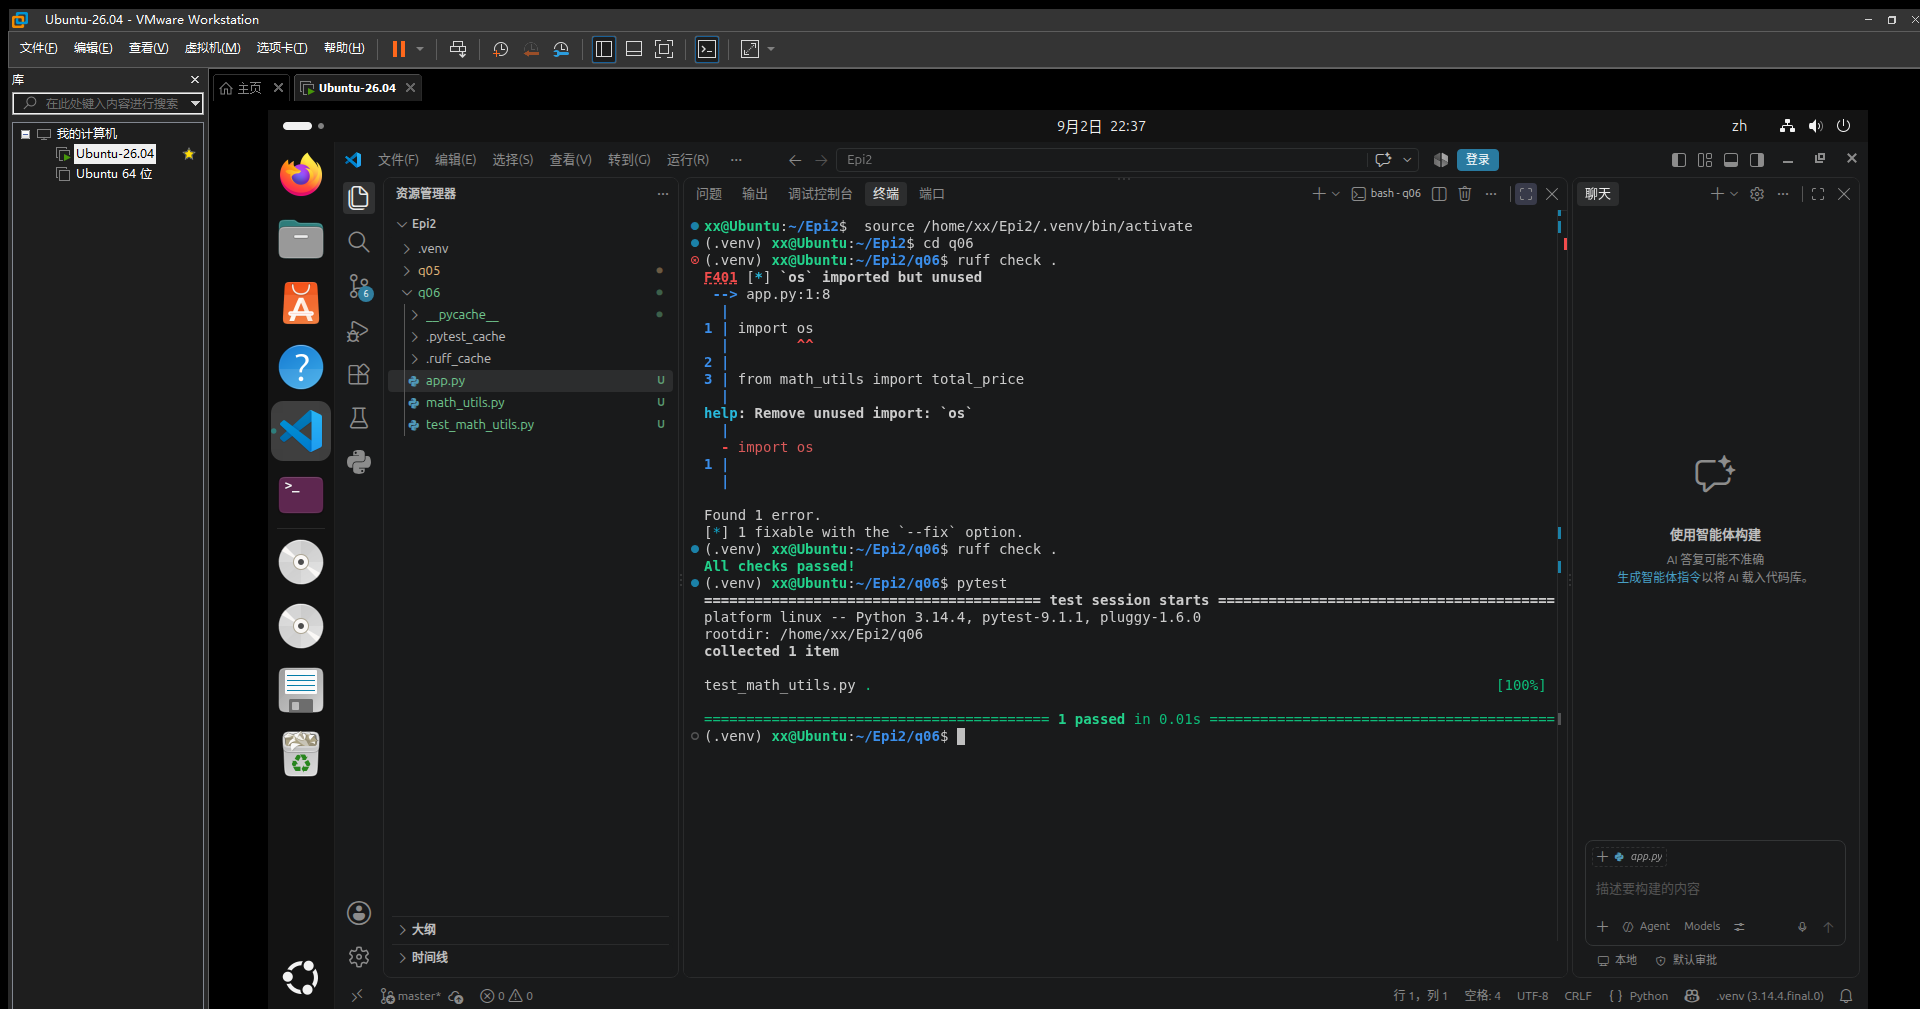
\includegraphics[width=6.65694in,height=3.95556in]{media/media/q06_3.png}

\vspace{0.6em}
\textbf{五、解题感悟}

1. 这次第一次比较完整地用到了语言服务器的功能，发现跳转定义和查找引用在代码多起来以后会方便很多。

2. 直接修改函数名容易漏掉其他地方的引用，使用重命名符号可以一起修改，感觉比手动搜索更可靠。

3. ruff 和 pytest 一个检查代码问题，一个检查程序功能，最后一起运行可以更早发现问题，平时写代码也可以养成这个习惯。

\vspace{1em}
\textbf{第7题：用调试器定位归并排序缺陷}

\vspace{0.6em}
\textbf{一、主题}

Debugging

\vspace{0.6em}
\textbf{二、题目要求}

1. 将给定的归并排序代码保存到 q07/merge\_sort.py，先运行给定输入，确认程序结果错误或出现异常。

2. 使用 pdb、IDE Debugger 或其他调试器，在 merge 函数中设置断点，并观察 i、j、left[i] 和 right[j] 的变化。

3. 找到代码中的错误并进行最小修改，不得直接使用 sorted 替换归并排序。

4. 使用 pytest 增加两个测试，分别测试题目给定的输入和含有重复元素的列表，并保证测试全部通过。

\vspace{0.6em}
\textbf{三、源程序代码}

无

\vspace{0.6em}
\textbf{四、程序运行结果}

debug：

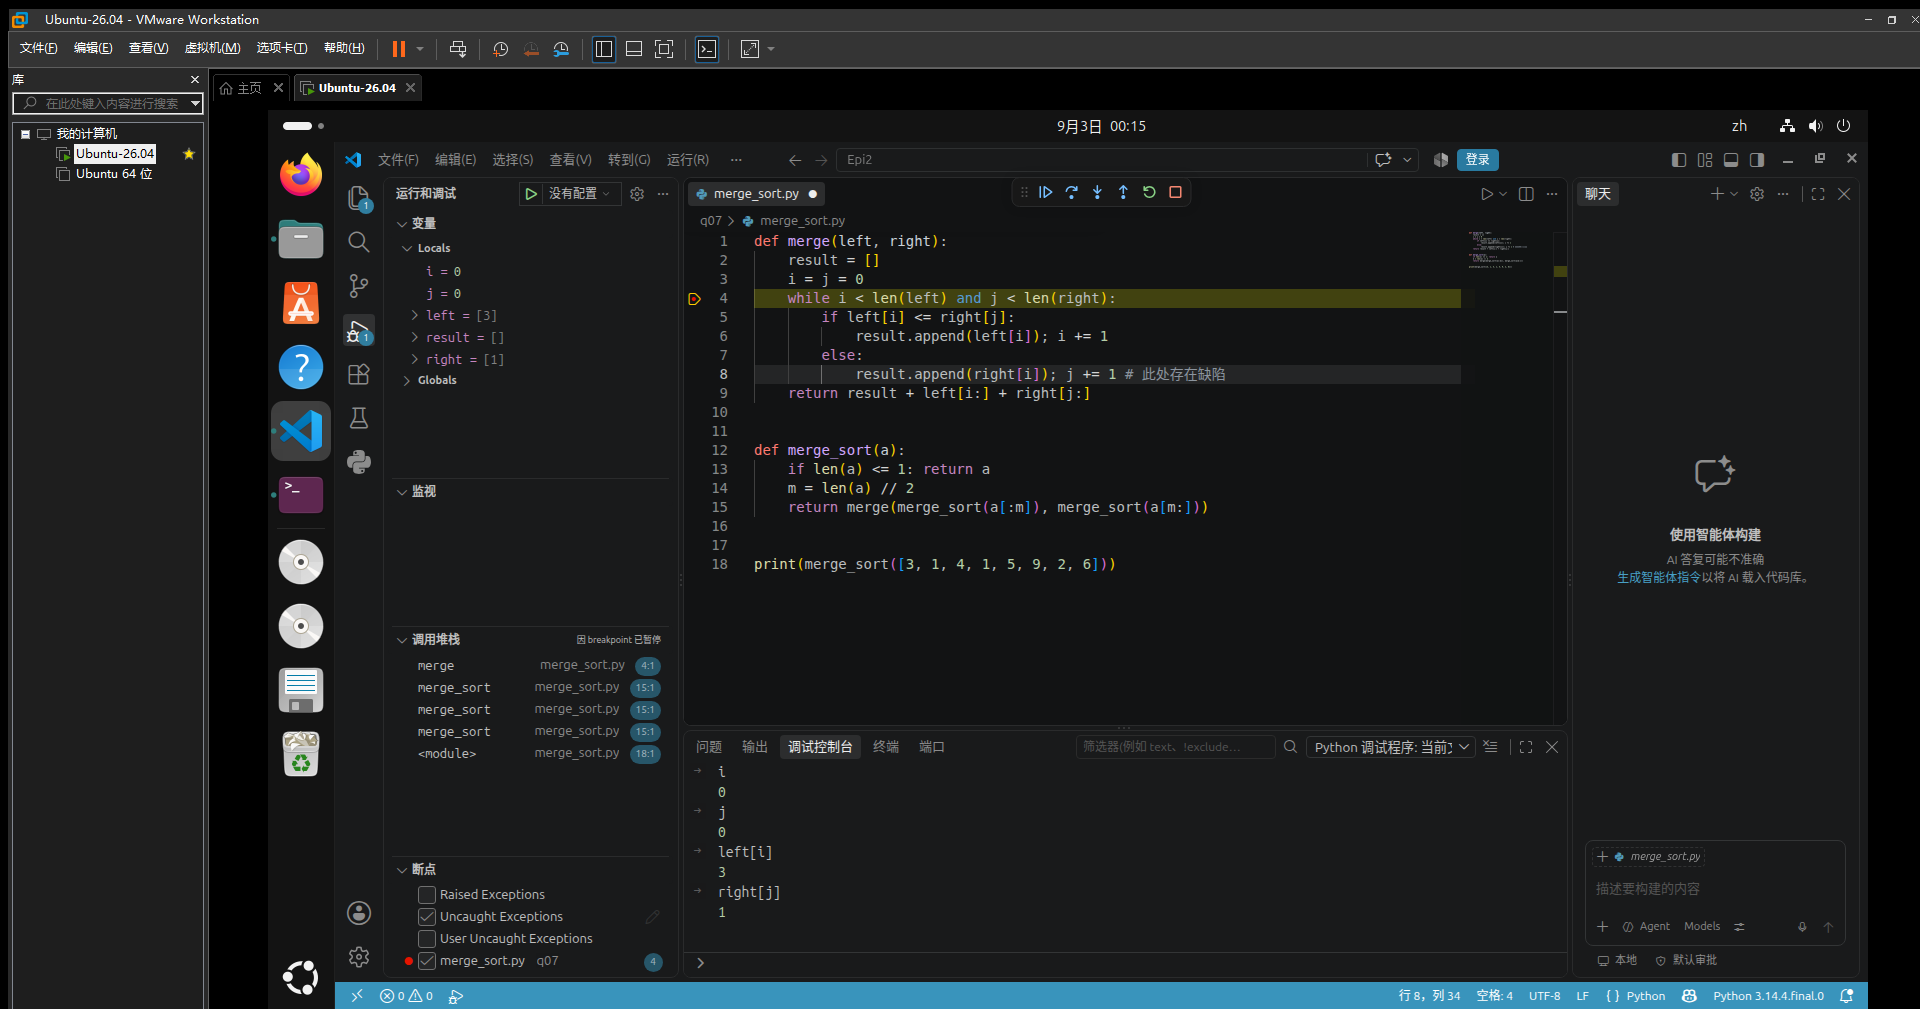
\includegraphics[width=6.65694in,height=3.95556in]{media/media/q07_1.png}

vscode运行结果：

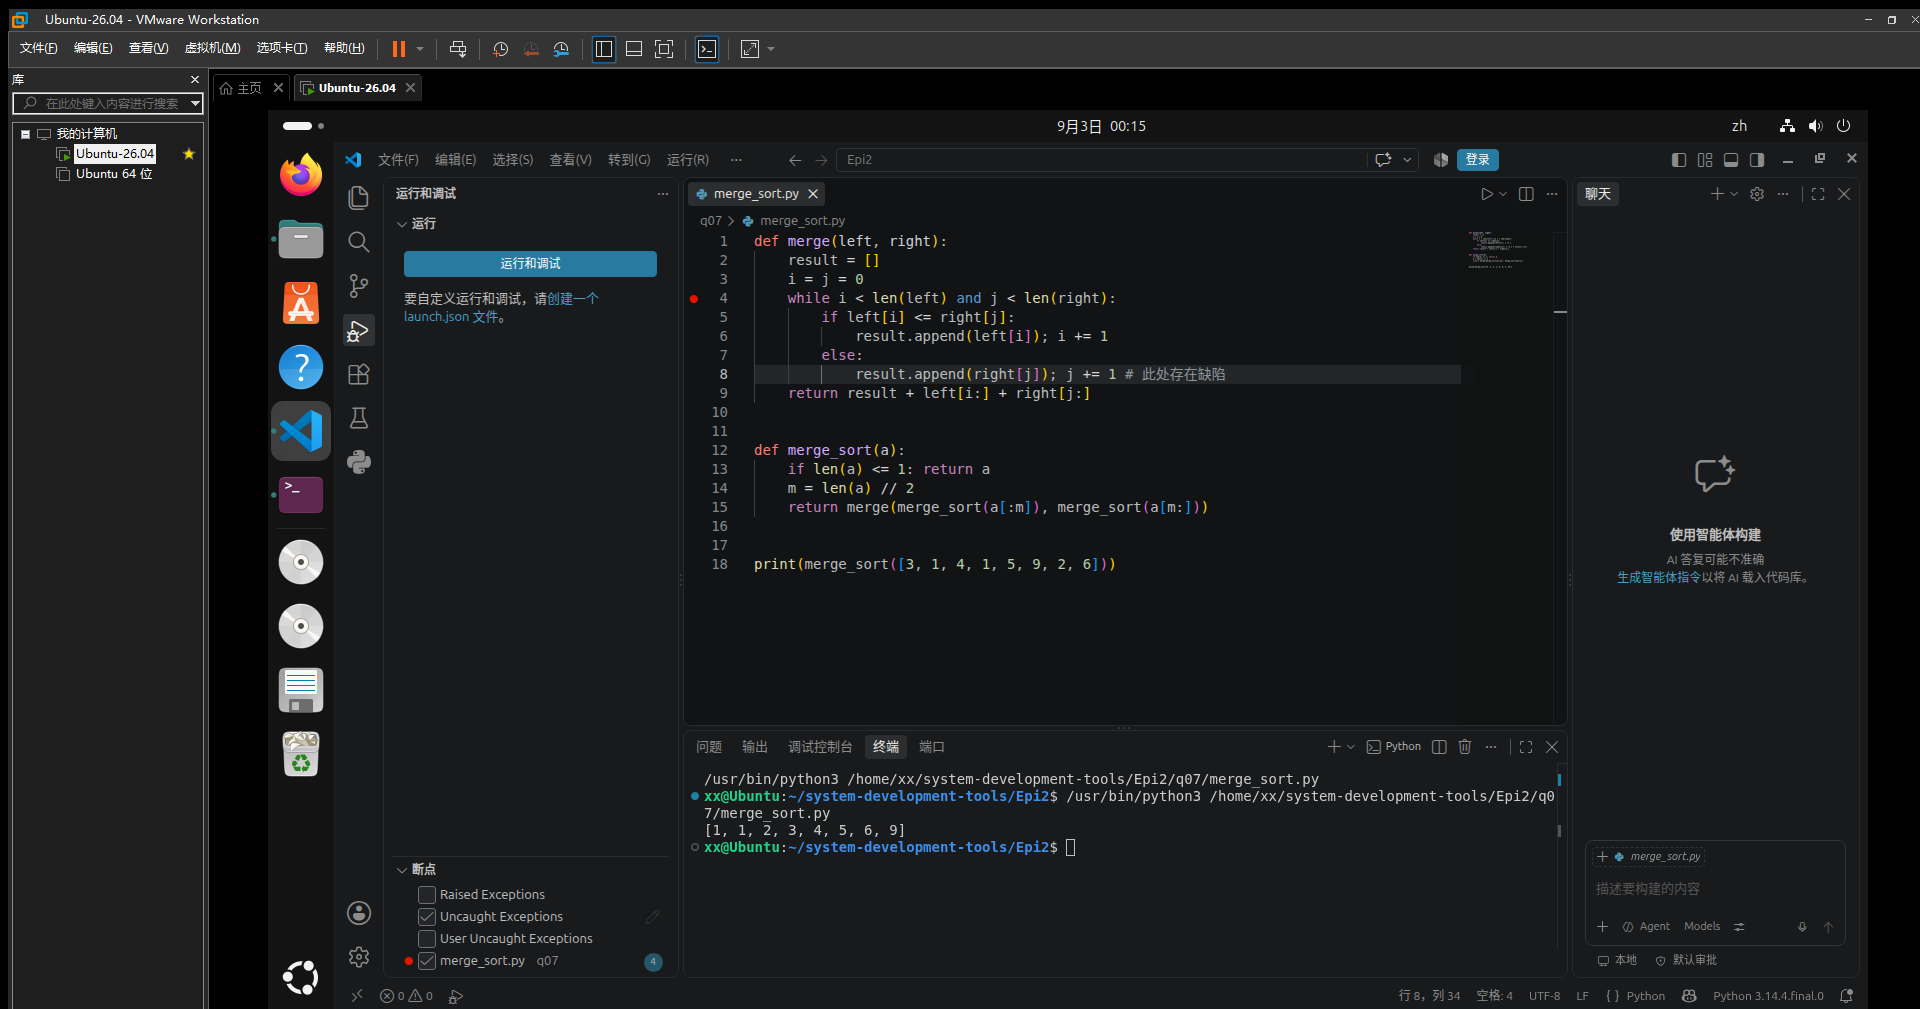
\includegraphics[width=6.65694in,height=3.95556in]{media/media/q07_2.png}

pytest结果：

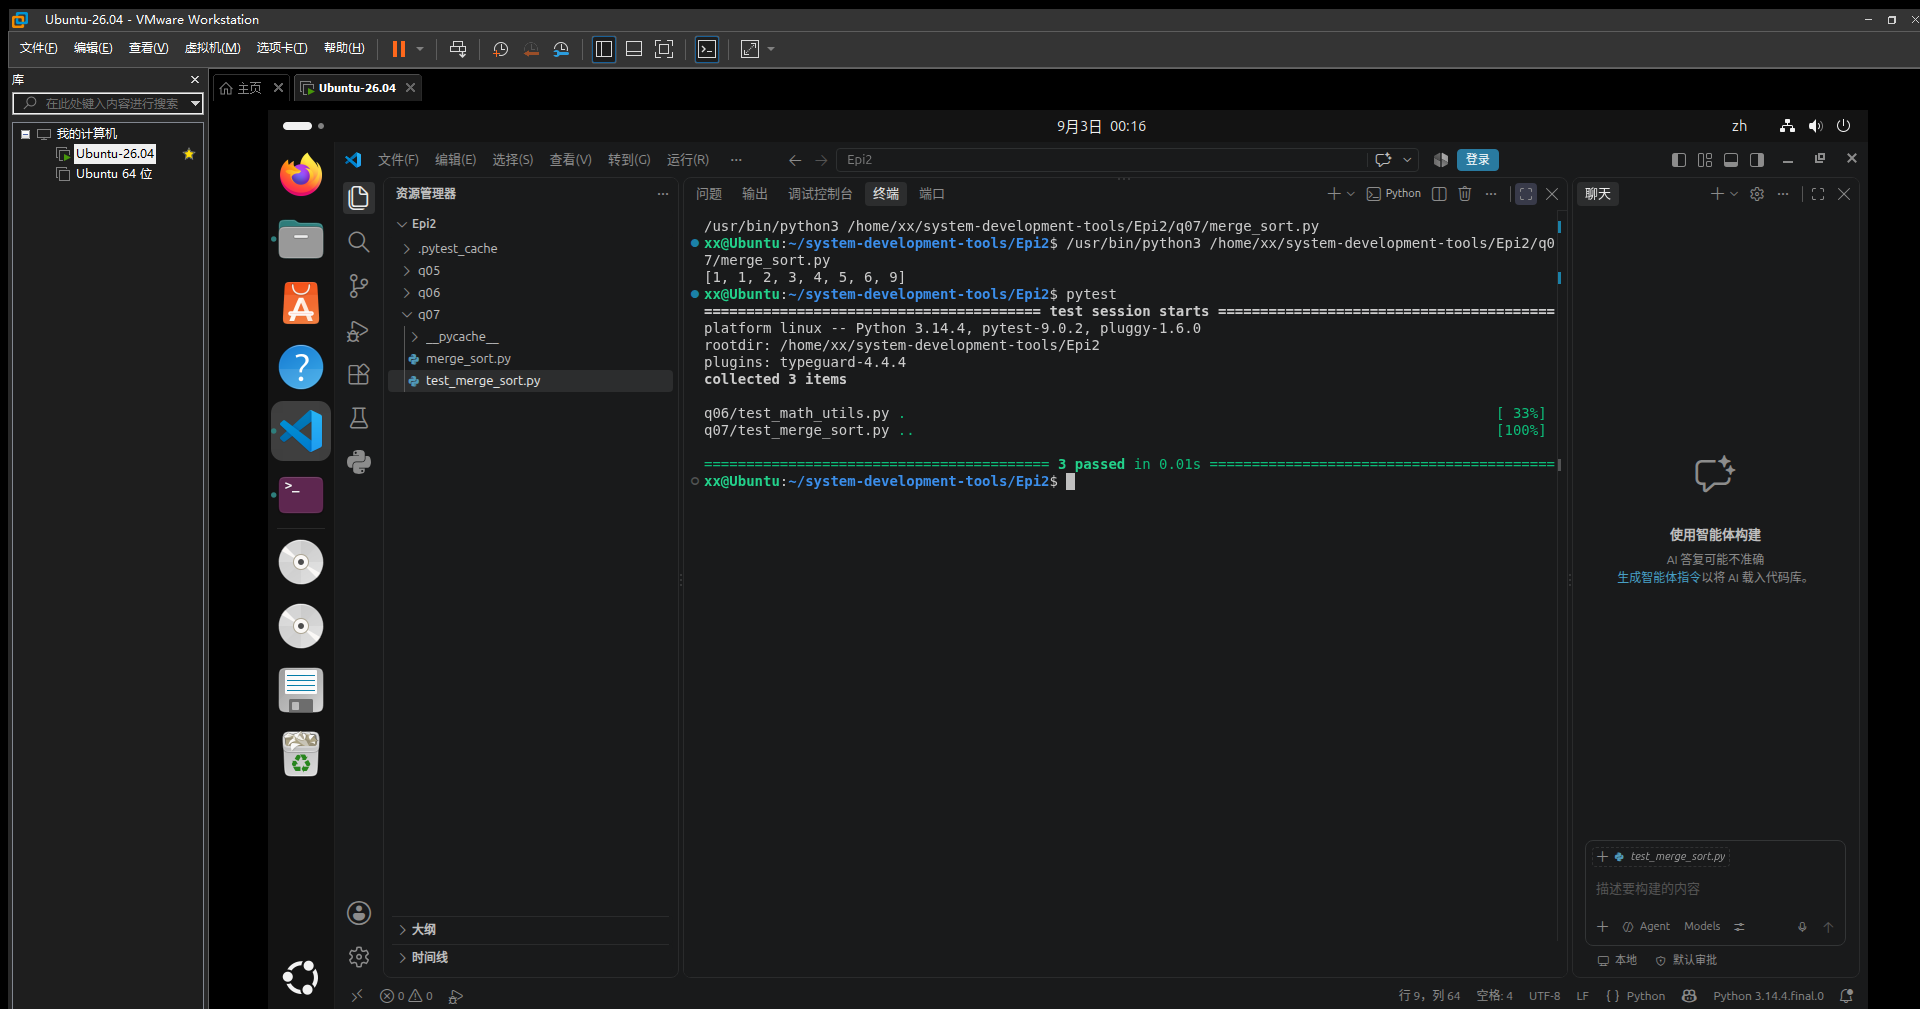
\includegraphics[width=6.65694in,height=3.95556in]{media/media/q07_3.png}

\vspace{0.6em}
\textbf{五、解题感悟}

1. 直接看代码的时候不太容易发现下标的问题，运行调试器后观察 i 和 j 的变化就比较容易定位错误。

2. 这次体会到断点调试比单纯加很多 print 更方便，可以直接看到程序运行到某一行时变量的具体状态。

3. 修复后再用 pytest 测试，比只运行一次程序更放心，也能检查包含重复元素的情况有没有问题。

\vspace{1em}
\textbf{第8题：先测量，再优化慢速词频程序}

\vspace{0.6em}
\textbf{一、主题}

Profiling

\vspace{0.6em}
\textbf{二、题目要求}

1. 在 q08 中创建 generate\_words.py 和 wordfreq.py，运行生成程序得到固定的 words.txt。

2. 使用 time 运行原始词频程序两次，记录每次运行耗时。

3. 使用 cProfile -s cumulative 运行一次程序，根据分析结果找出主要耗时位置。

4. 在不改变最终 count 的情况下优化程序，不能直接把 1000 写死。

5. 使用相同的 words.txt 再运行优化后的程序两次，记录耗时，并计算优化前后的中位数和加速比。

\vspace{0.6em}
\textbf{三、源程序代码}

无

\vspace{0.6em}
\textbf{四、程序运行结果}

vscode结果：

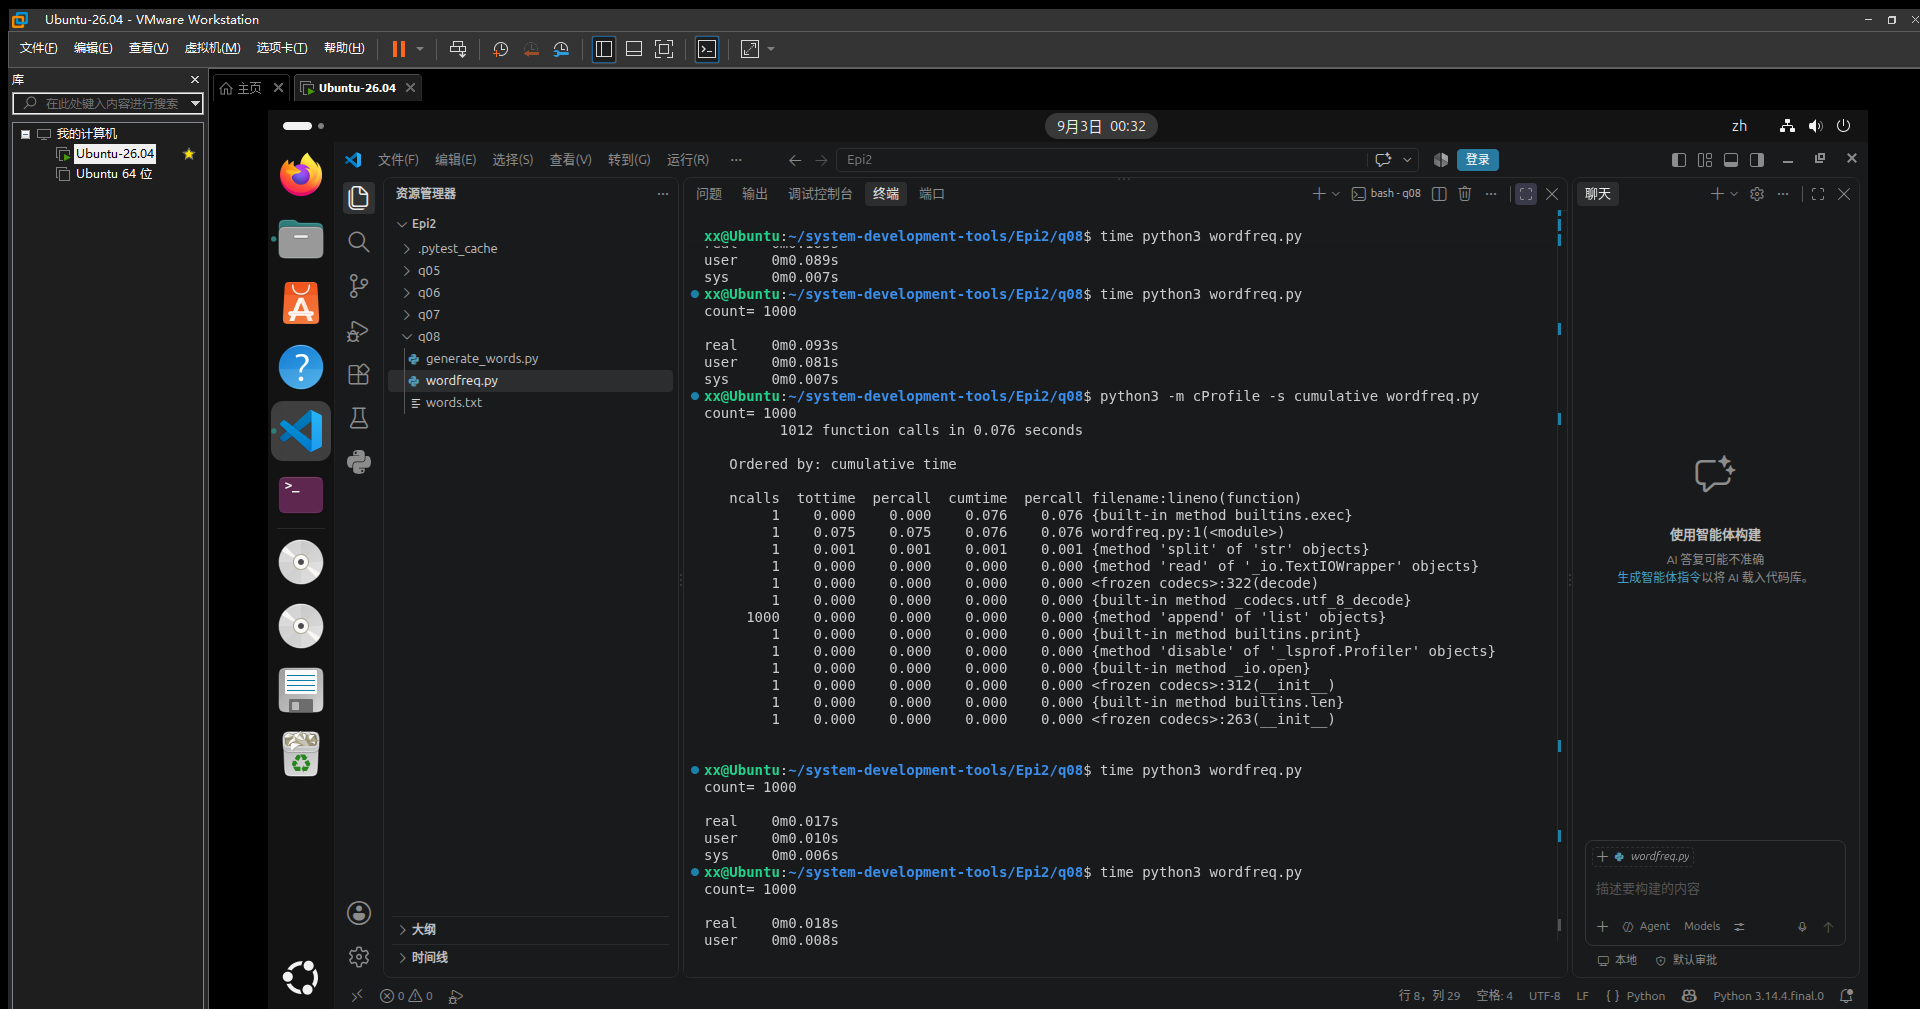
\includegraphics[width=6.65694in,height=3.95556in]{media/media/q08_1.png}

项目     优化前     优化后

第一次     0.105 s     0.017 s

第二次     0.093 s     0.018 s

中位数     0.099 s     0.0175 s

count     1000     1000

加速比     —     约 5.66×

\vspace{0.6em}
\textbf{五、解题感悟}

1. 这次发现程序能正常运行不代表效率就好，原程序虽然结果正确，但是使用列表查找重复单词会花费很多时间。

2. 通过 cProfile 可以先找到程序比较慢的地方，再决定怎么修改，而不是凭感觉乱优化。

3. 优化后 count 还是 1000，但运行时间明显降低，说明使用合适的数据结构对程序效率影响还是很大的。

\textbf{课后练习}

\vspace{1em}
\textbf{练习1：处理以 - 开头的文件名}

\vspace{0.6em}
\textbf{一、主题}

命令行环境

\vspace{0.6em}
\textbf{二、题目要求}

你可能见过像 cmd -{}-flag -{}- -{}-notaflag 这样的命令。这里的 -{}- 是一个特殊参数，它告诉程序后面不要再继续解析选项（flag）了。也就是说，-{}- 后面的所有内容都会被当作位置参数（positional argument）。这有什么用？试着运行 touch -{}- -myfile，然后在不使用 -{}- 的情况下把它删掉。

\vspace{0.6em}
\textbf{三、源程序代码}

touch -{}- -myfile

ls -l -{}- -myfile

rm -myfile

rm ./-myfile

ls -l ./-myfile

\vspace{0.6em}
\textbf{四、程序运行结果}

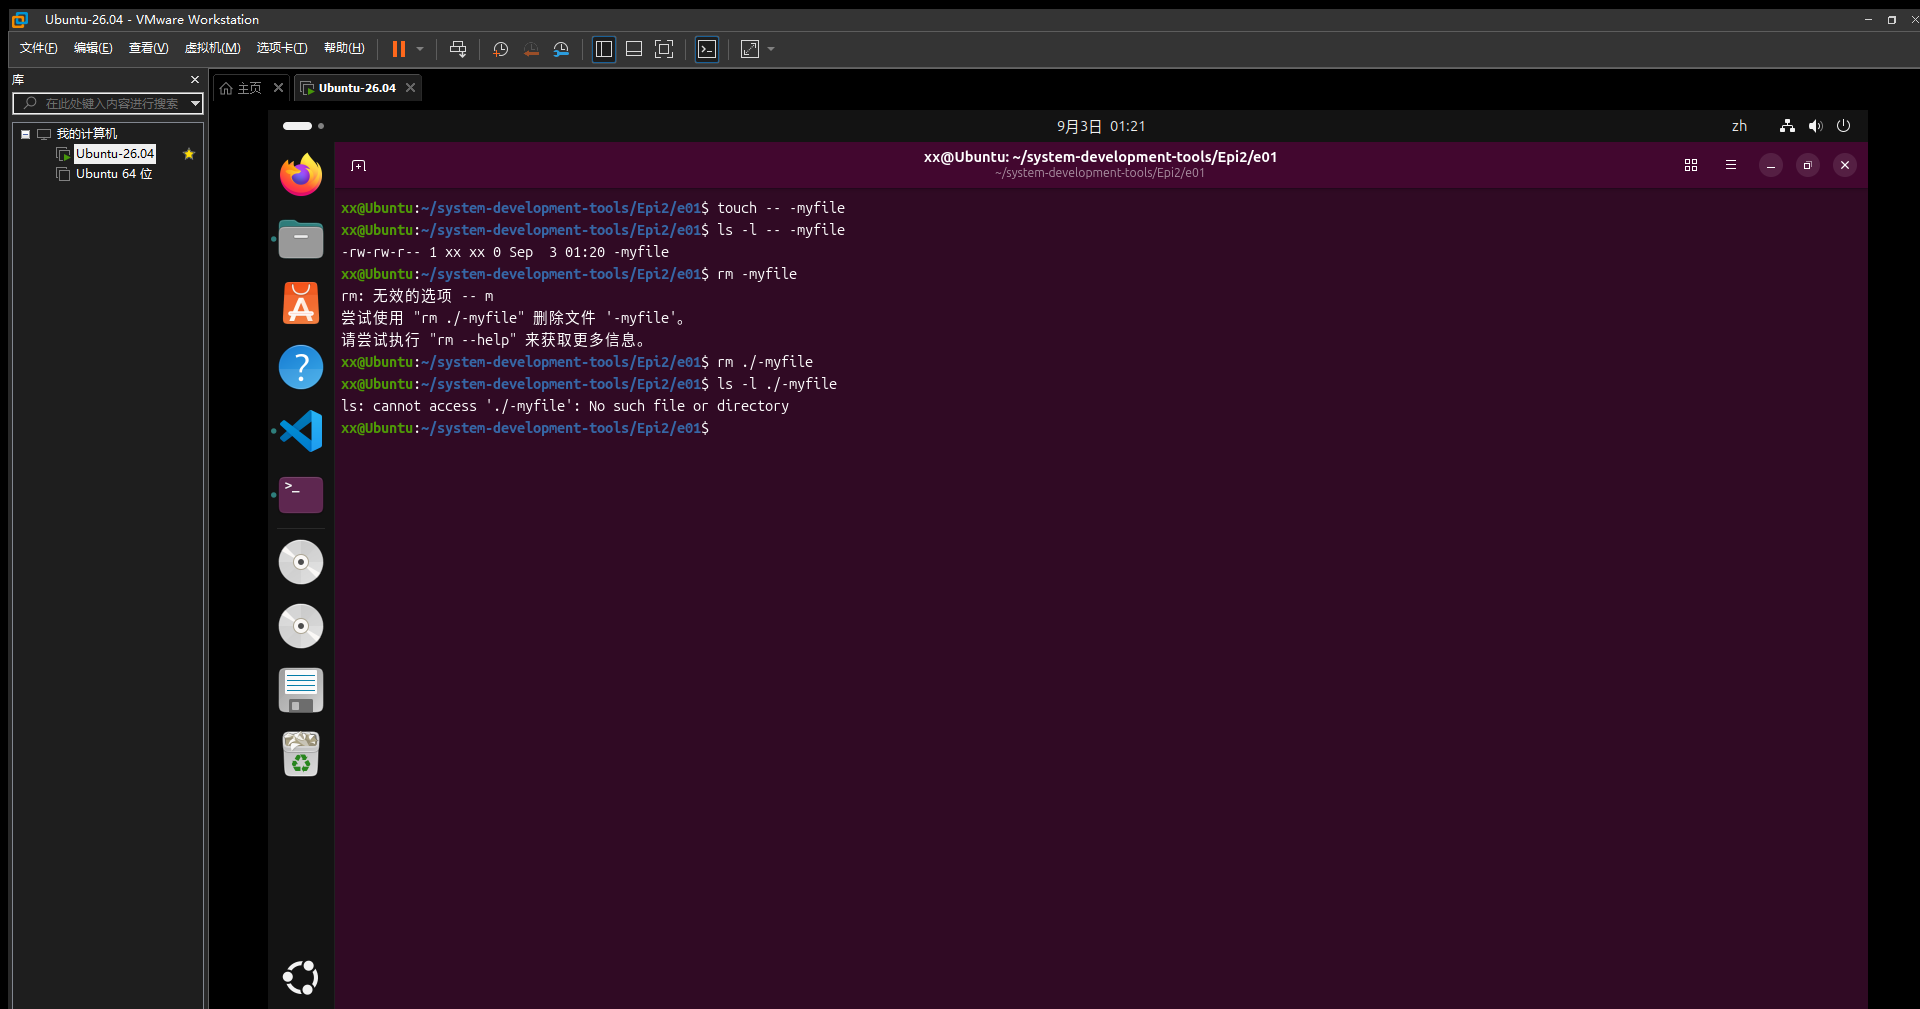
\includegraphics[width=6.65694in,height=3.95556in]{media/media/e01_1.png}

\vspace{0.6em}
\textbf{五、解题感悟}

1. 以前没注意到文件名以 - 开头时会被当成命令选项。

2. -{}- 可以让命令停止解析后面的选项。

3. 使用 ./-myfile 也可以正常处理这种文件名。

\vspace{1em}
\textbf{练习2：组合 ls 参数查看文件信息}

\vspace{0.6em}
\textbf{一、主题}

命令行环境

\vspace{0.6em}
\textbf{二、题目要求}

编写一条命令，列出当前目录中的所有文件，包括隐藏文件，以人类可读的格式显示，按照修改时间排序，并使用彩色输出。

\vspace{0.6em}
\textbf{三、源程序代码}

touch test.txt

ls -laht -{}-color=auto

\vspace{0.6em}
\textbf{四、程序运行结果}

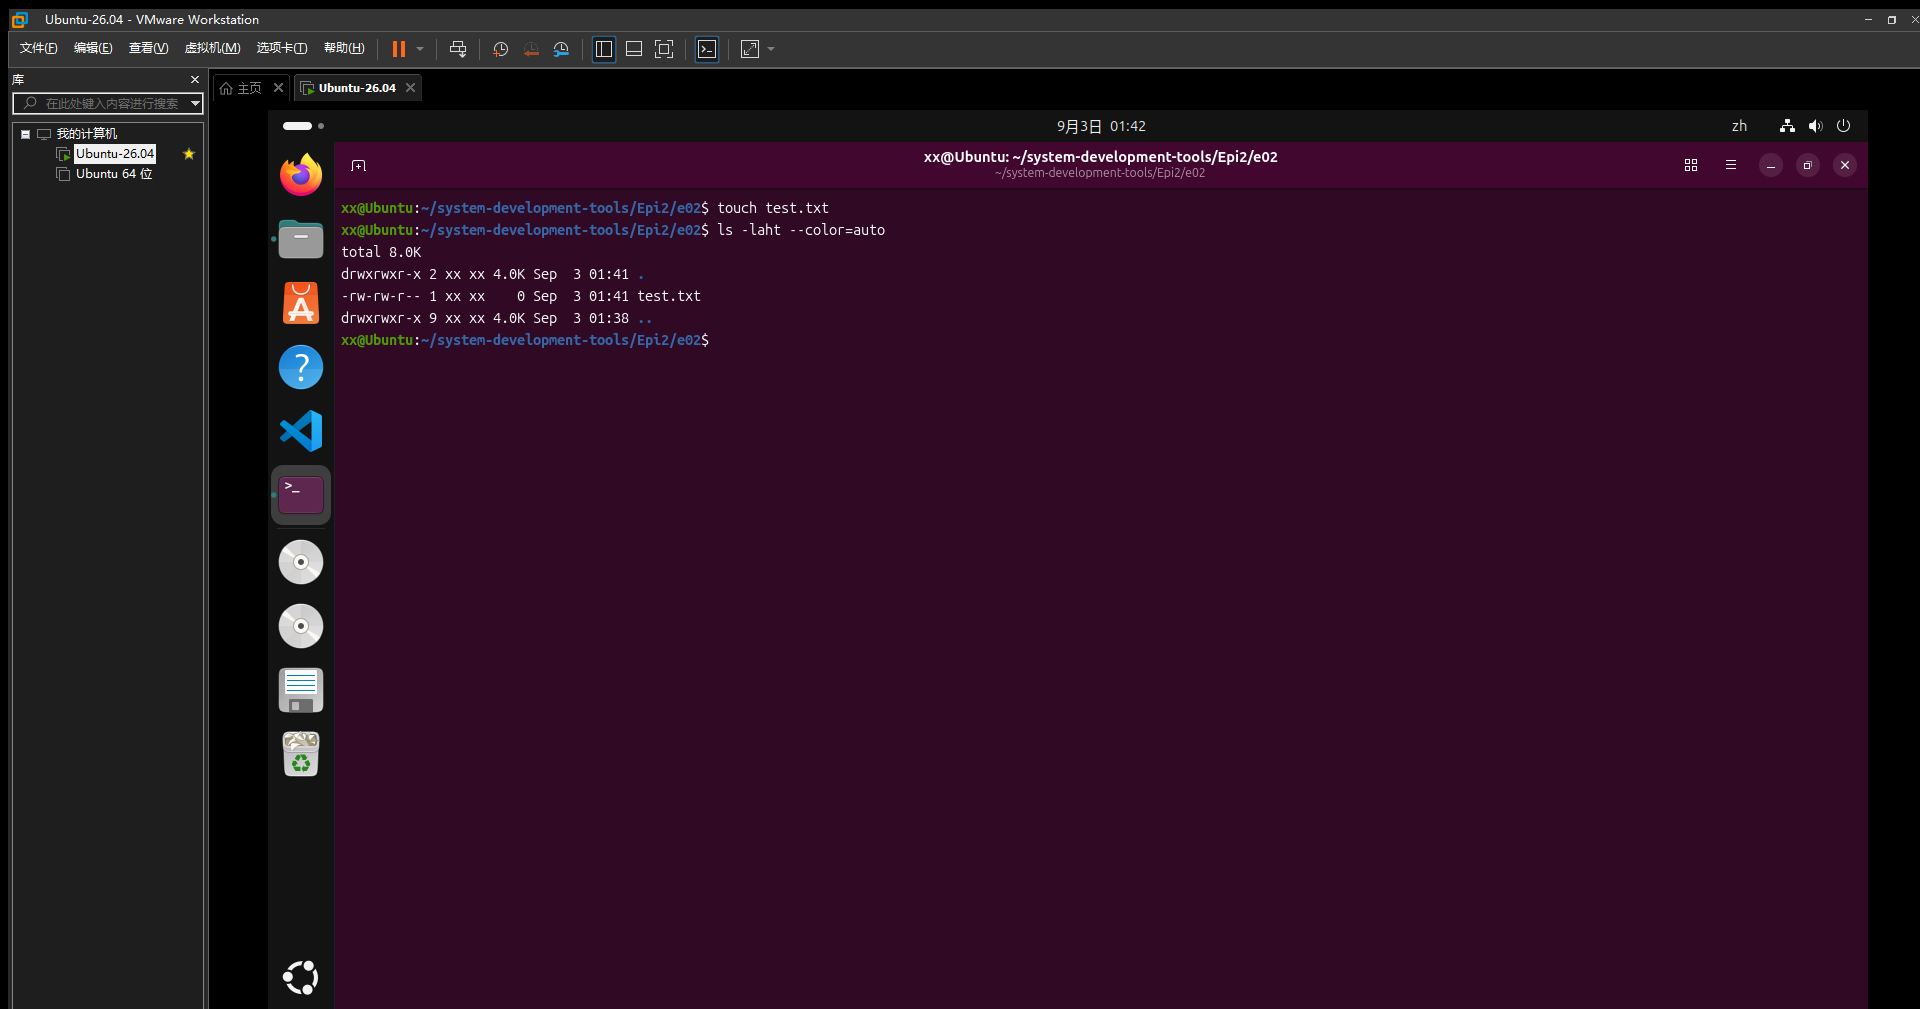
\includegraphics[width=6.65694in,height=3.95556in]{media/media/e02_1.png}

\vspace{0.6em}
\textbf{五、解题感悟}

1. 这题主要是把几个 ls 参数组合起来使用。

2. -a 可以显示平时看不到的隐藏文件。

3. -t 可以按照修改时间排序，-h 让文件大小更容易看懂。

\vspace{1em}
\textbf{练习3：为 cd 创建别名}

\vspace{0.6em}
\textbf{一、主题}

命令行环境

\vspace{0.6em}
\textbf{二、题目要求}

创建一个别名，使运行 dc 时能够执行 cd，以防止不小心将 cd 输入成 dc。

\vspace{0.6em}
\textbf{三、源程序代码}

alias dc=cd

pwd

dc ..

pwd

\vspace{0.6em}
\textbf{四、程序运行结果}

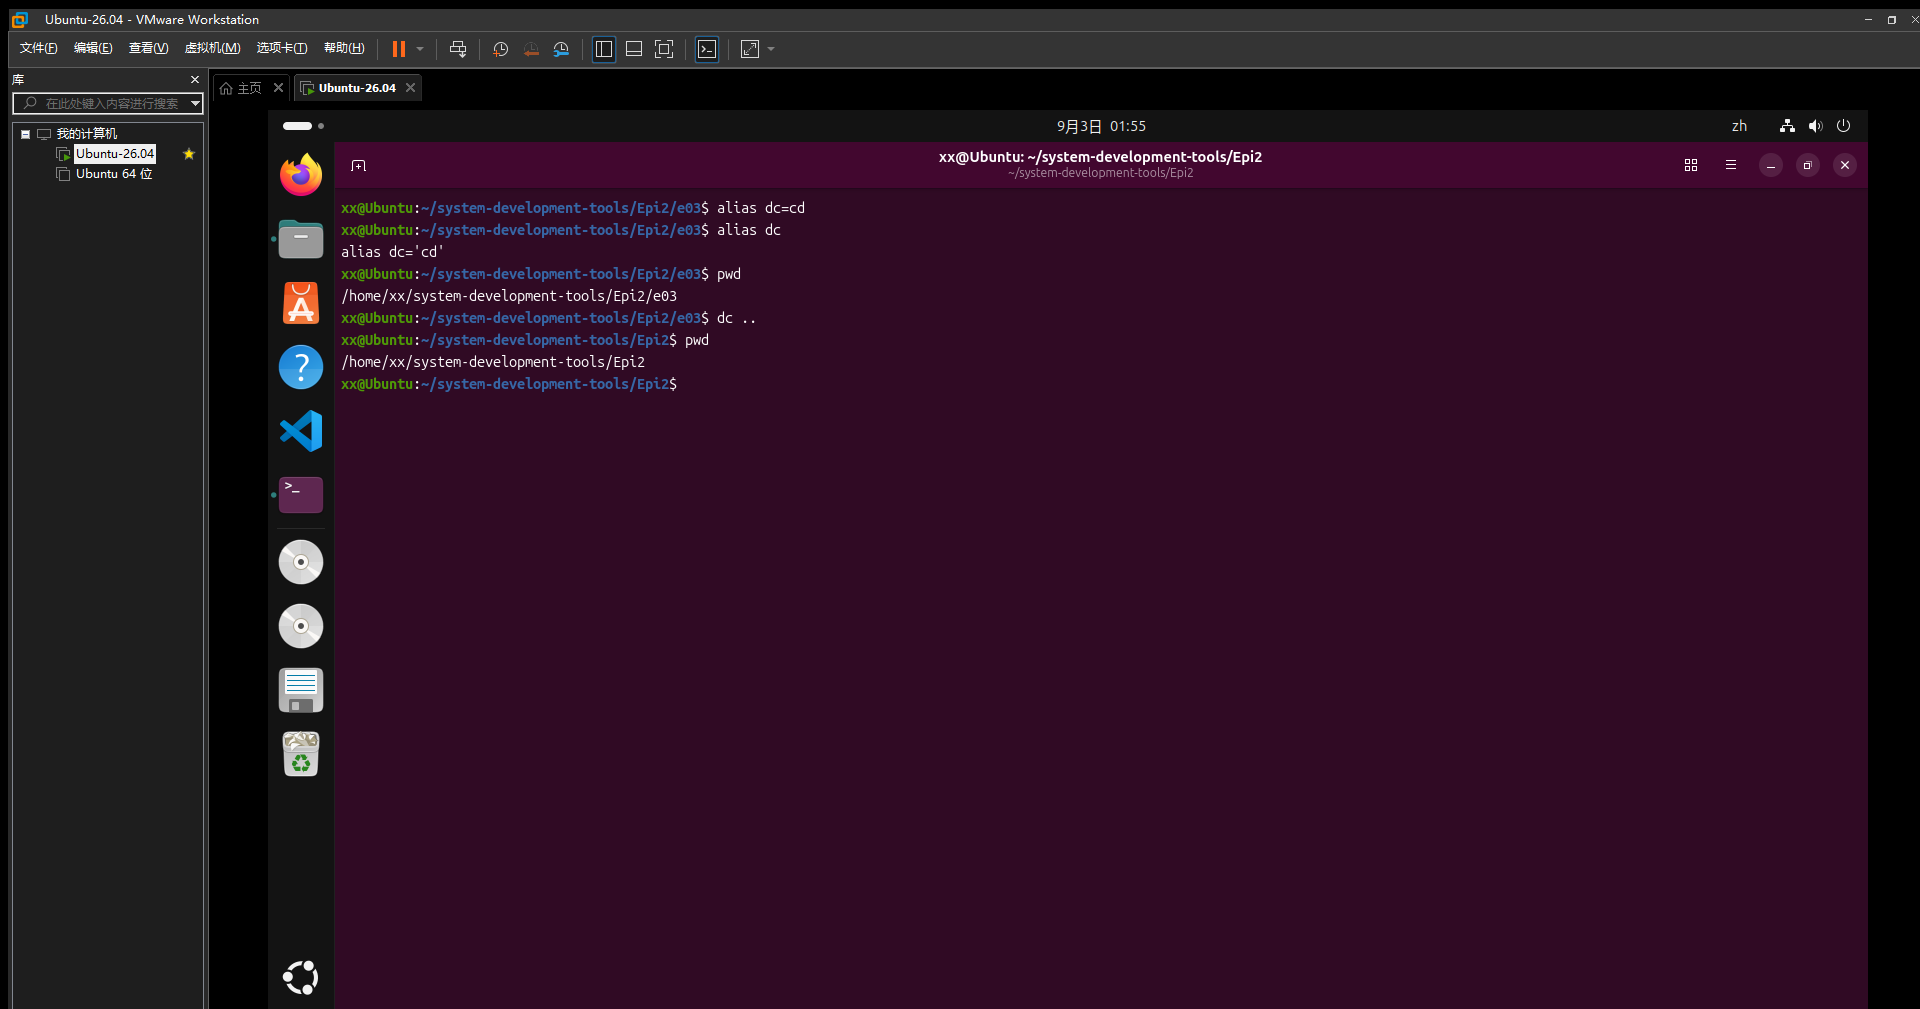
\includegraphics[width=6.65694in,height=3.95556in]{media/media/e03_1.png}

\vspace{0.6em}
\textbf{五、解题感悟}

1. alias 可以给命令设置一个简短的名字。

2. 我用 dc .. 测试后，发现它确实执行了 cd ..。

3. 这次使用的是临时 alias，关闭终端后就会失效。

\vspace{1em}
\textbf{练习4：配置 IDE 扩展与语言服务器}

\vspace{0.6em}
\textbf{一、主题}

开发环境与工具

\vspace{0.6em}
\textbf{二、题目要求}

为你正在做的一个项目配置 IDE 扩展和语言服务器。确保所有预期功能都能正常工作，例如对库依赖进行跳转到定义。如果你手头没有可用于这个练习的代码，也可以从 GitHub 上找一个开源项目来用。

\vspace{0.6em}
\textbf{三、源程序代码}

无

\vspace{0.6em}
\textbf{四、程序运行结果}

自动补全：

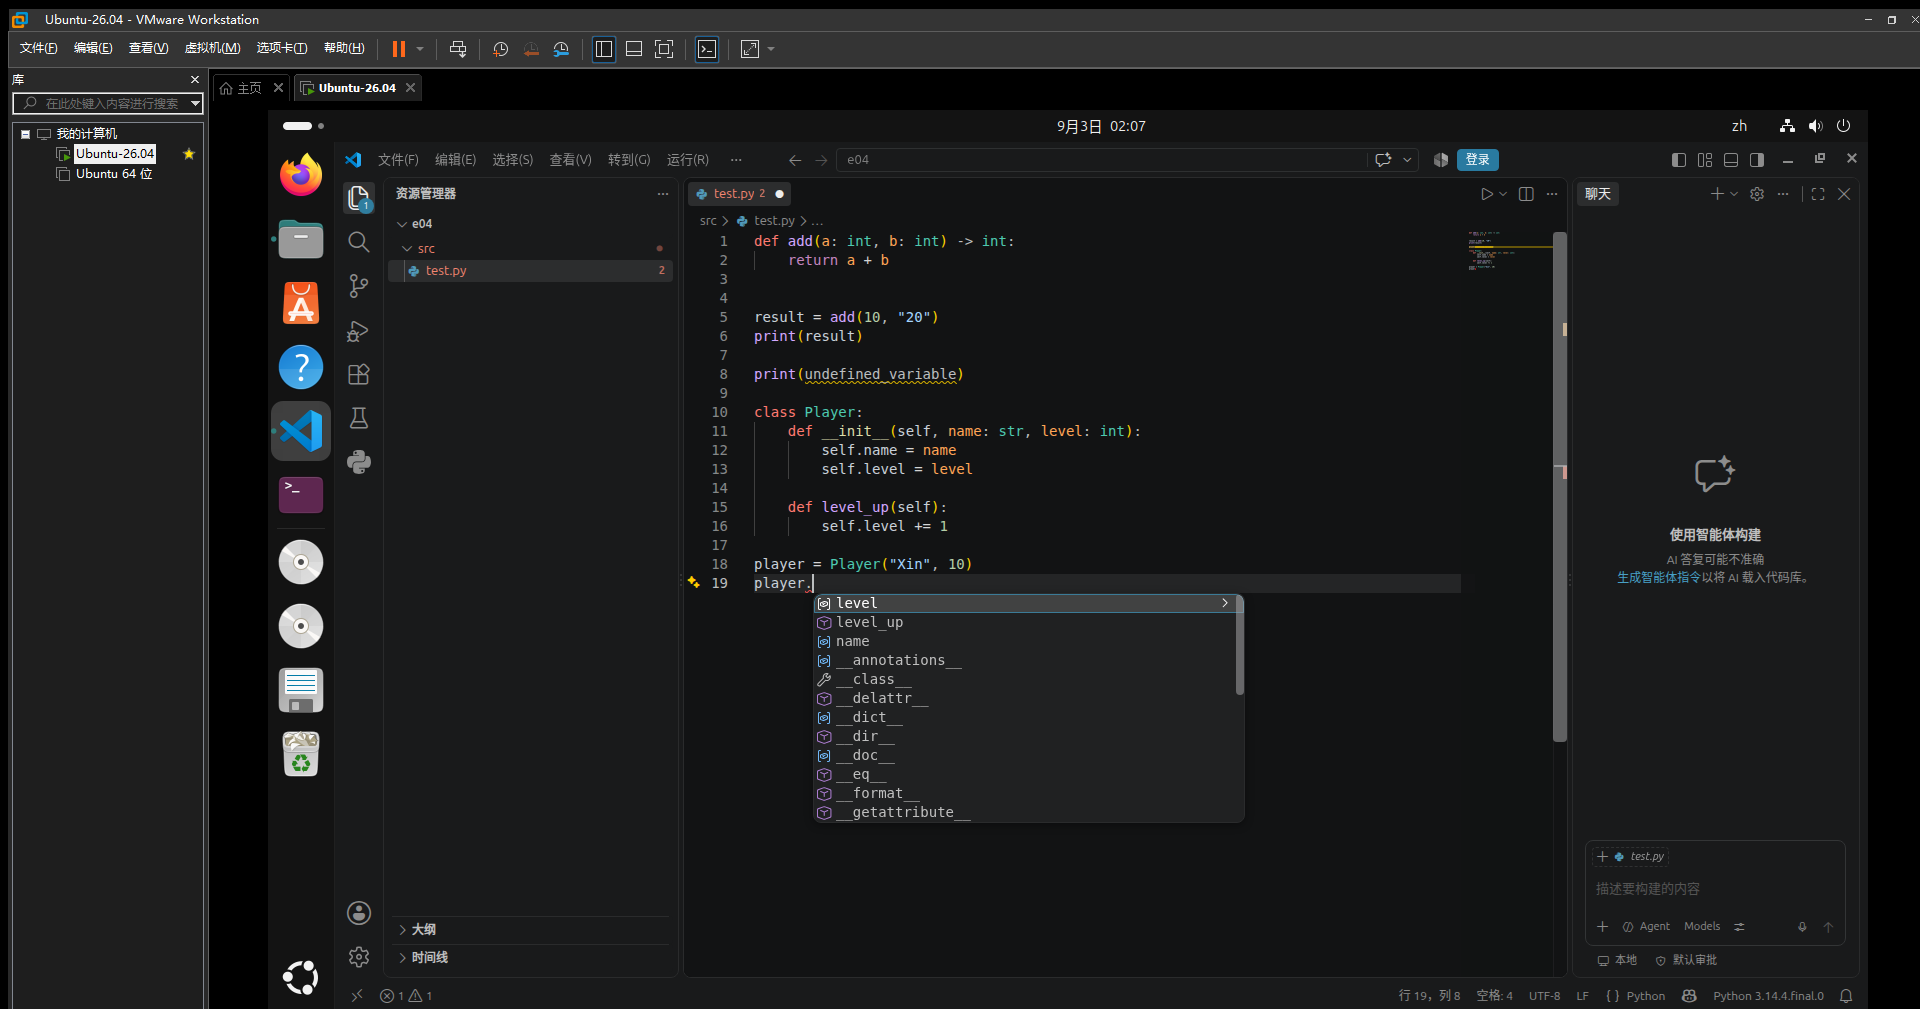
\includegraphics[width=6.65694in,height=3.95556in]{media/media/e04_1.png}

鼠标悬停问题检测：

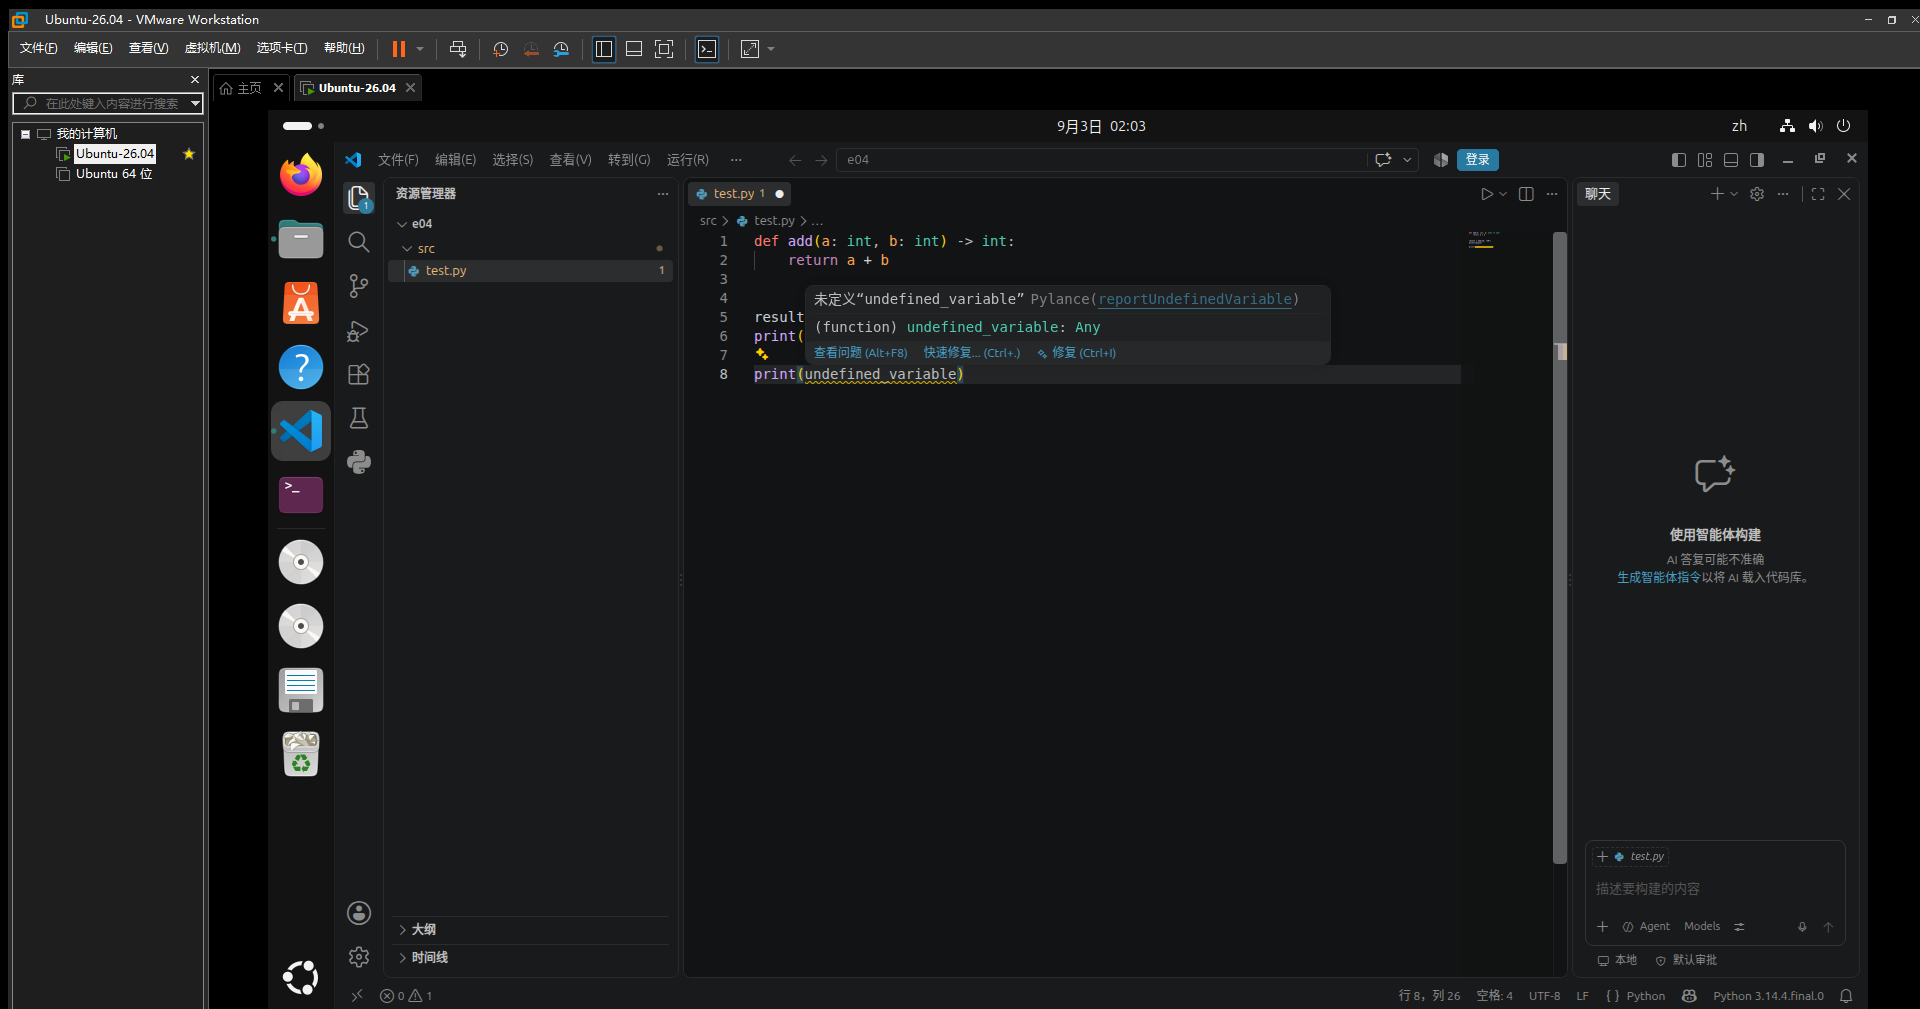
\includegraphics[width=6.65694in,height=3.95556in]{media/media/e04_2.png}

\vspace{0.6em}
\textbf{五、解题感悟}

1. 这次配置了 Python 的 IDE 扩展和 Pylance 语言服务器。

2. 体验了代码补全、类型检查和错误提示等功能。

3. 语言服务器可以帮助 IDE 更好地理解代码结构，提高编程效率。

\vspace{1em}
\textbf{练习5：安装实用的 IDE 扩展}

\vspace{0.6em}
\textbf{一、主题}

开发环境与工具

\vspace{0.6em}
\textbf{二、题目要求}

浏览一份 IDE 扩展列表，安装一个看起来对你有用的扩展。

\vspace{0.6em}
\textbf{三、源程序代码}

无

\vspace{0.6em}
\textbf{四、程序运行结果}

安装拓展：

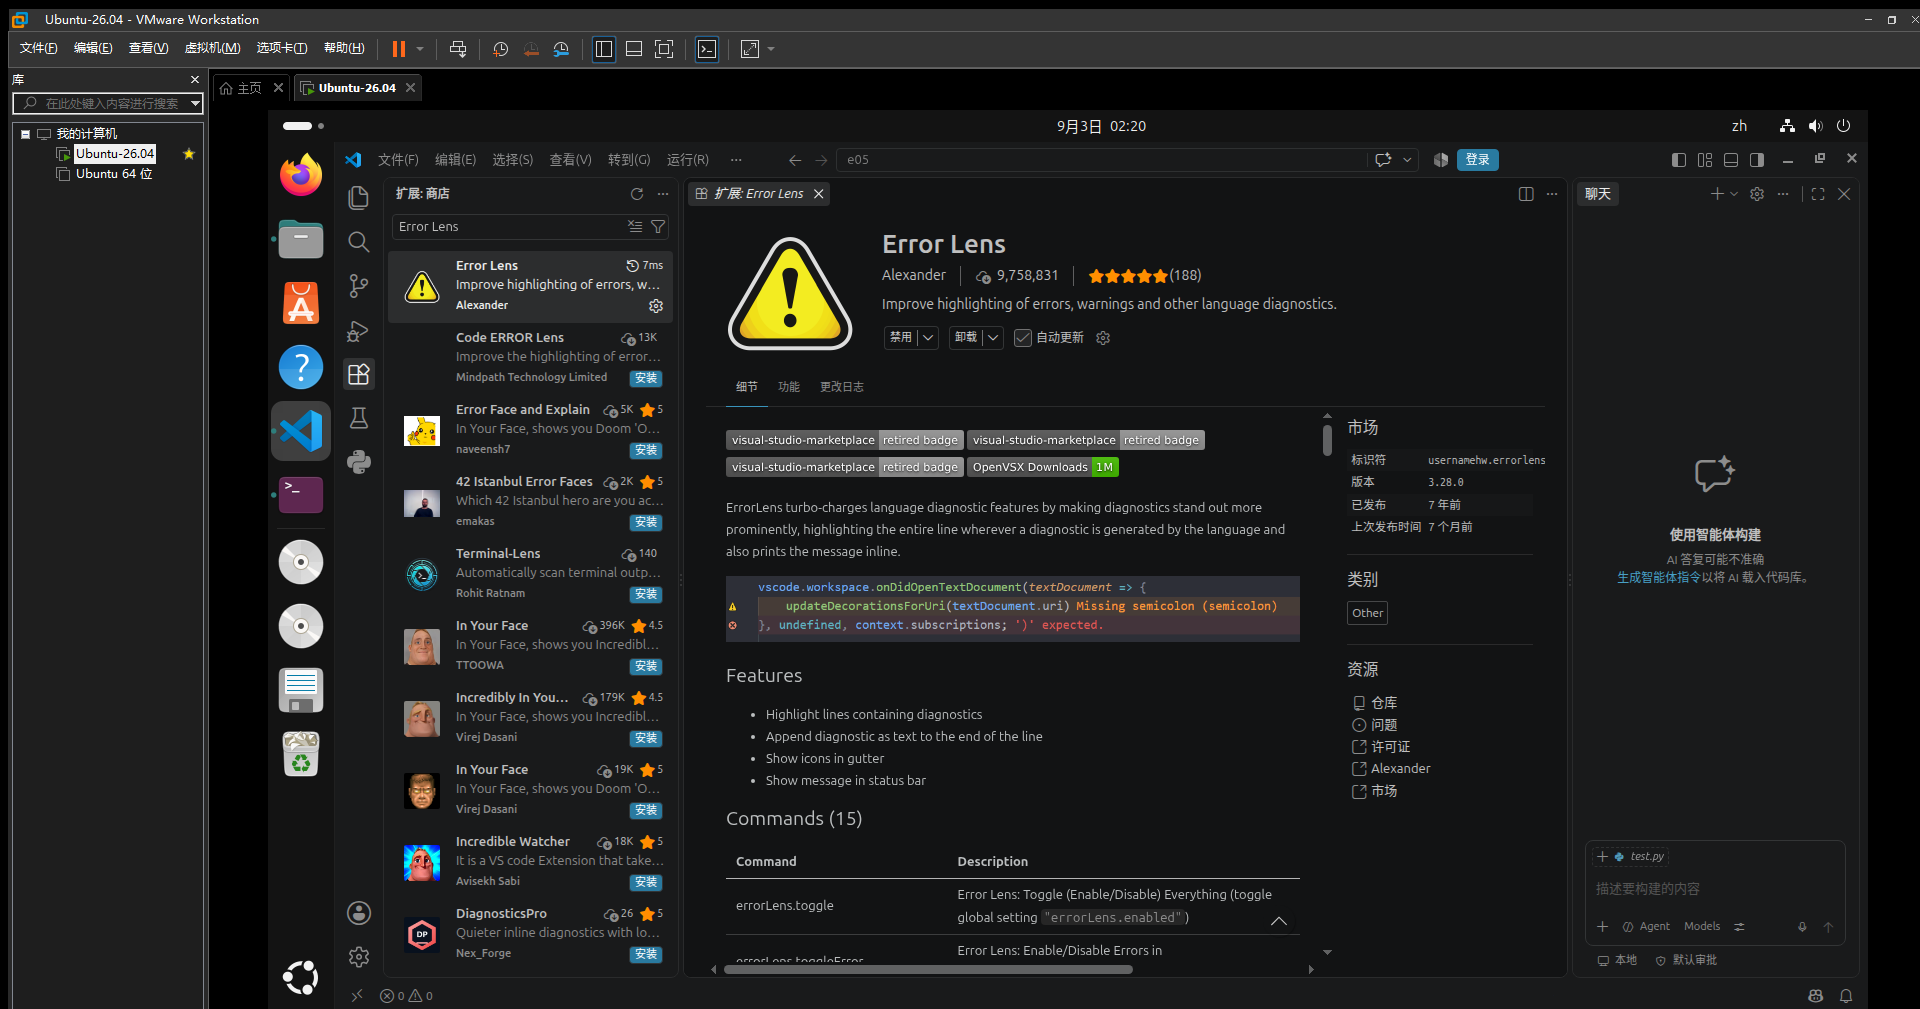
\includegraphics[width=6.65694in,height=3.95556in]{media/media/e05_1.png}

拓展效果：

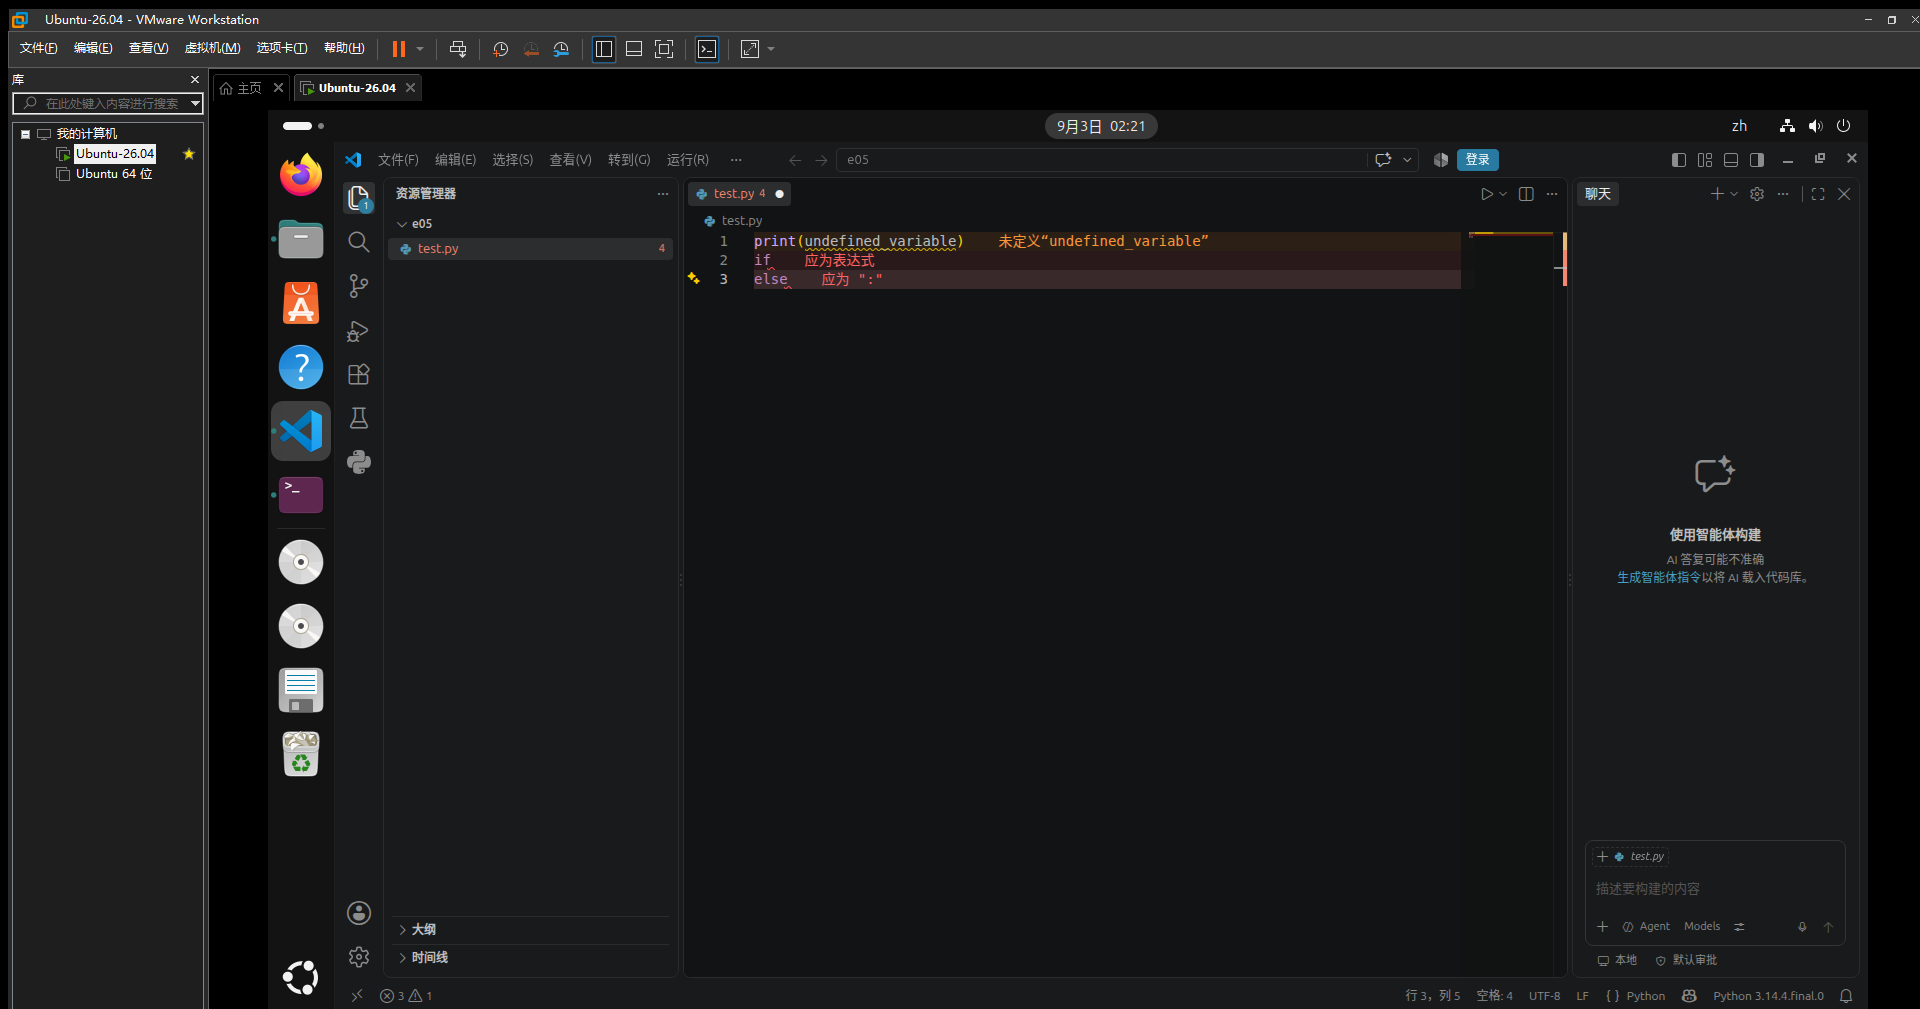
\includegraphics[width=6.65694in,height=3.95556in]{media/media/e05_2.png}

\vspace{0.6em}
\textbf{五、解题感悟}

1. 这次浏览了 VS Code 的扩展列表，并选择了 Error Lens。

2. Error Lens 可以直接在代码旁边显示错误和警告信息。

3. 安装扩展后，IDE 的使用体验更加方便。

\vspace{1em}
\textbf{练习6：VimGolf——Even and Odd}

\vspace{0.6em}
\textbf{一、主题}

开发环境与工具

\vspace{0.6em}
\textbf{二、题目要求}

将文件中的数字 0 到 99 重新排列为两行：第一行包含所有偶数，第二行包含所有奇数。每行中的数字按照从小到大的顺序排列，并以空格分隔。

\vspace{0.6em}
\textbf{三、源程序代码}

:\%d

:put =join(range(0,98,2))

:put =join(range(1,99,2))

:wq

\vspace{0.6em}
\textbf{四、程序运行结果}

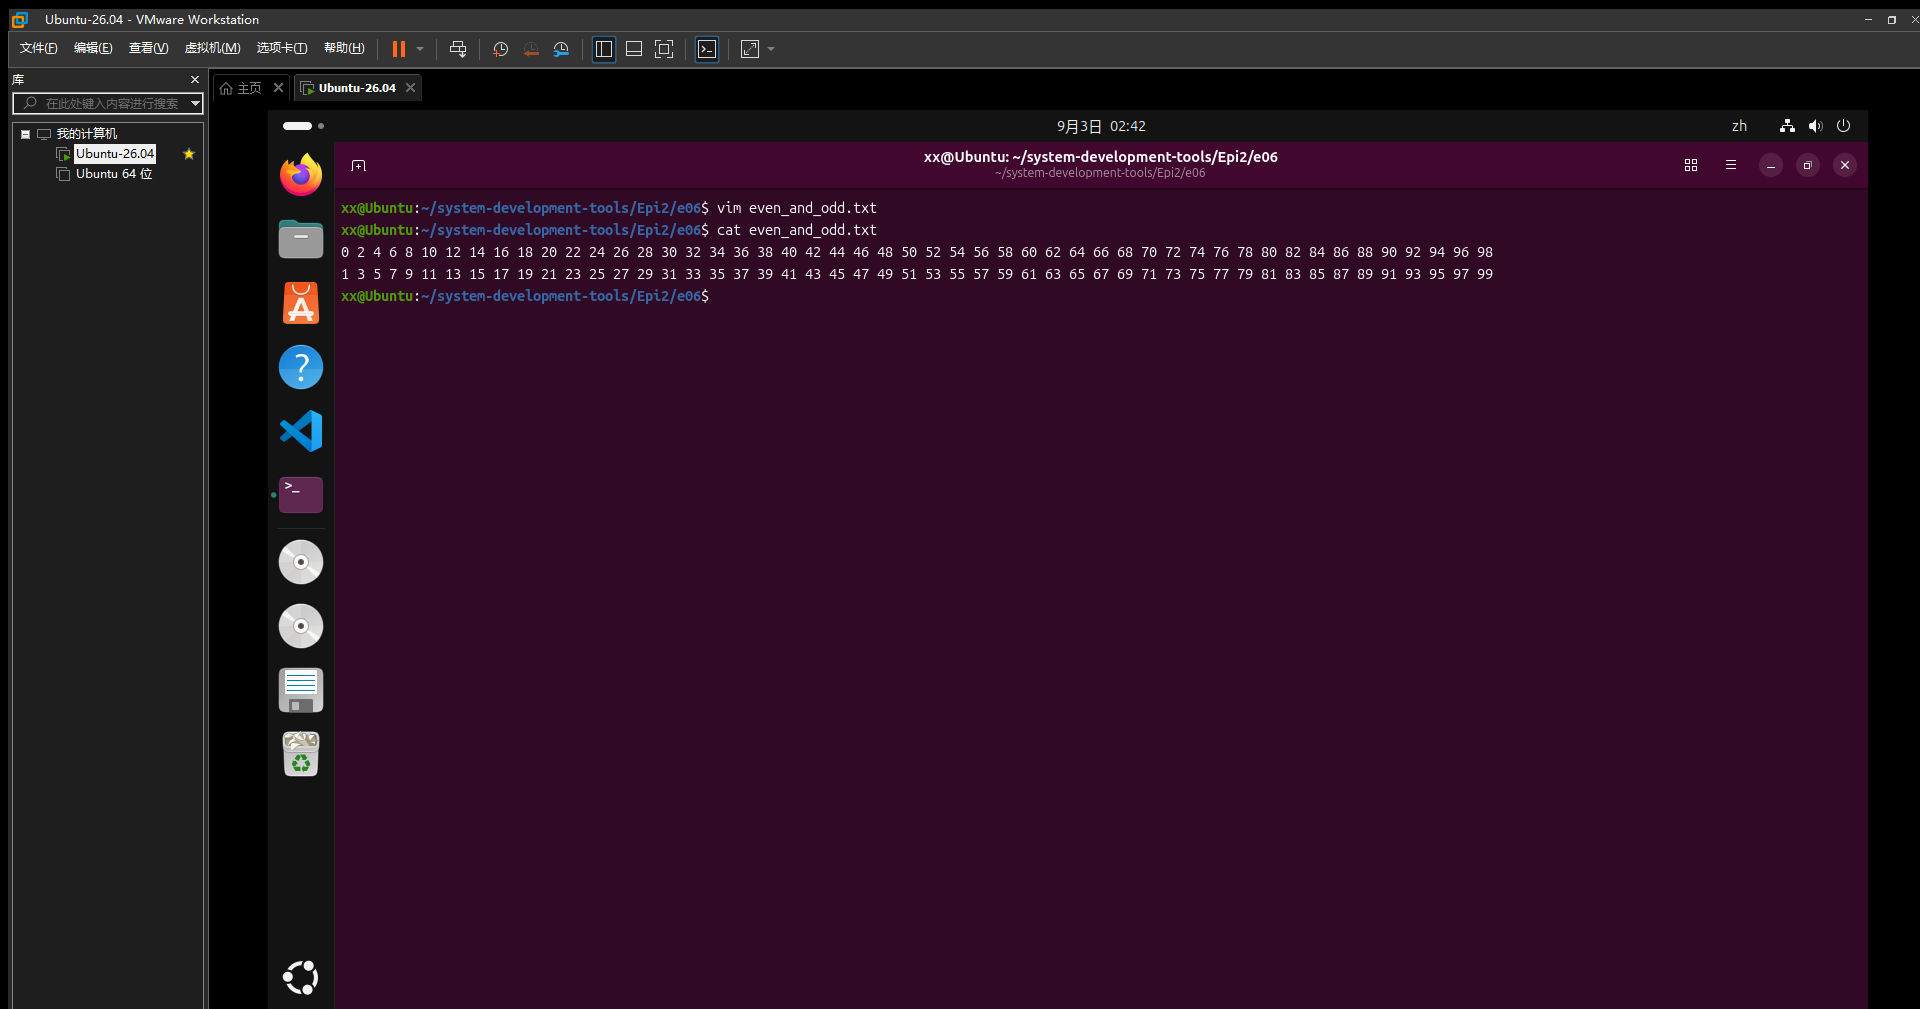
\includegraphics[width=6.65694in,height=3.95556in]{media/media/e06_1.png}

\vspace{0.6em}
\textbf{五、解题感悟}

1. 这次练习了 Vim 的命令模式和表达式寄存器。

2. range() 可以快速生成指定范围和步长的数字。

3. 用 Vim 的命令处理大量文本比手动修改快很多。

\vspace{1em}
\textbf{练习7：使用 AddressSanitizer 调试内存错误}

\vspace{0.6em}
\textbf{一、主题}

调试与性能分析

\vspace{0.6em}
\textbf{二、题目要求}

使用 AddressSanitizer（ASan）检测程序中的内存错误。编译并运行存在内存错误的程序，观察 AddressSanitizer 给出的错误信息，并根据错误提示定位和修复问题。

\vspace{0.6em}
\textbf{三、源程序代码}

vim uaf.c

gcc -g uaf.c -o uaf

./uaf

gcc -fsanitize=address -g uaf.c -o uaf\_asan

./uaf\_asan

vim uaf.c

gcc -fsanitize=address -g uaf.c -o uaf\_asan

./uaf\_asan

\vspace{0.6em}
\textbf{四、程序运行结果}

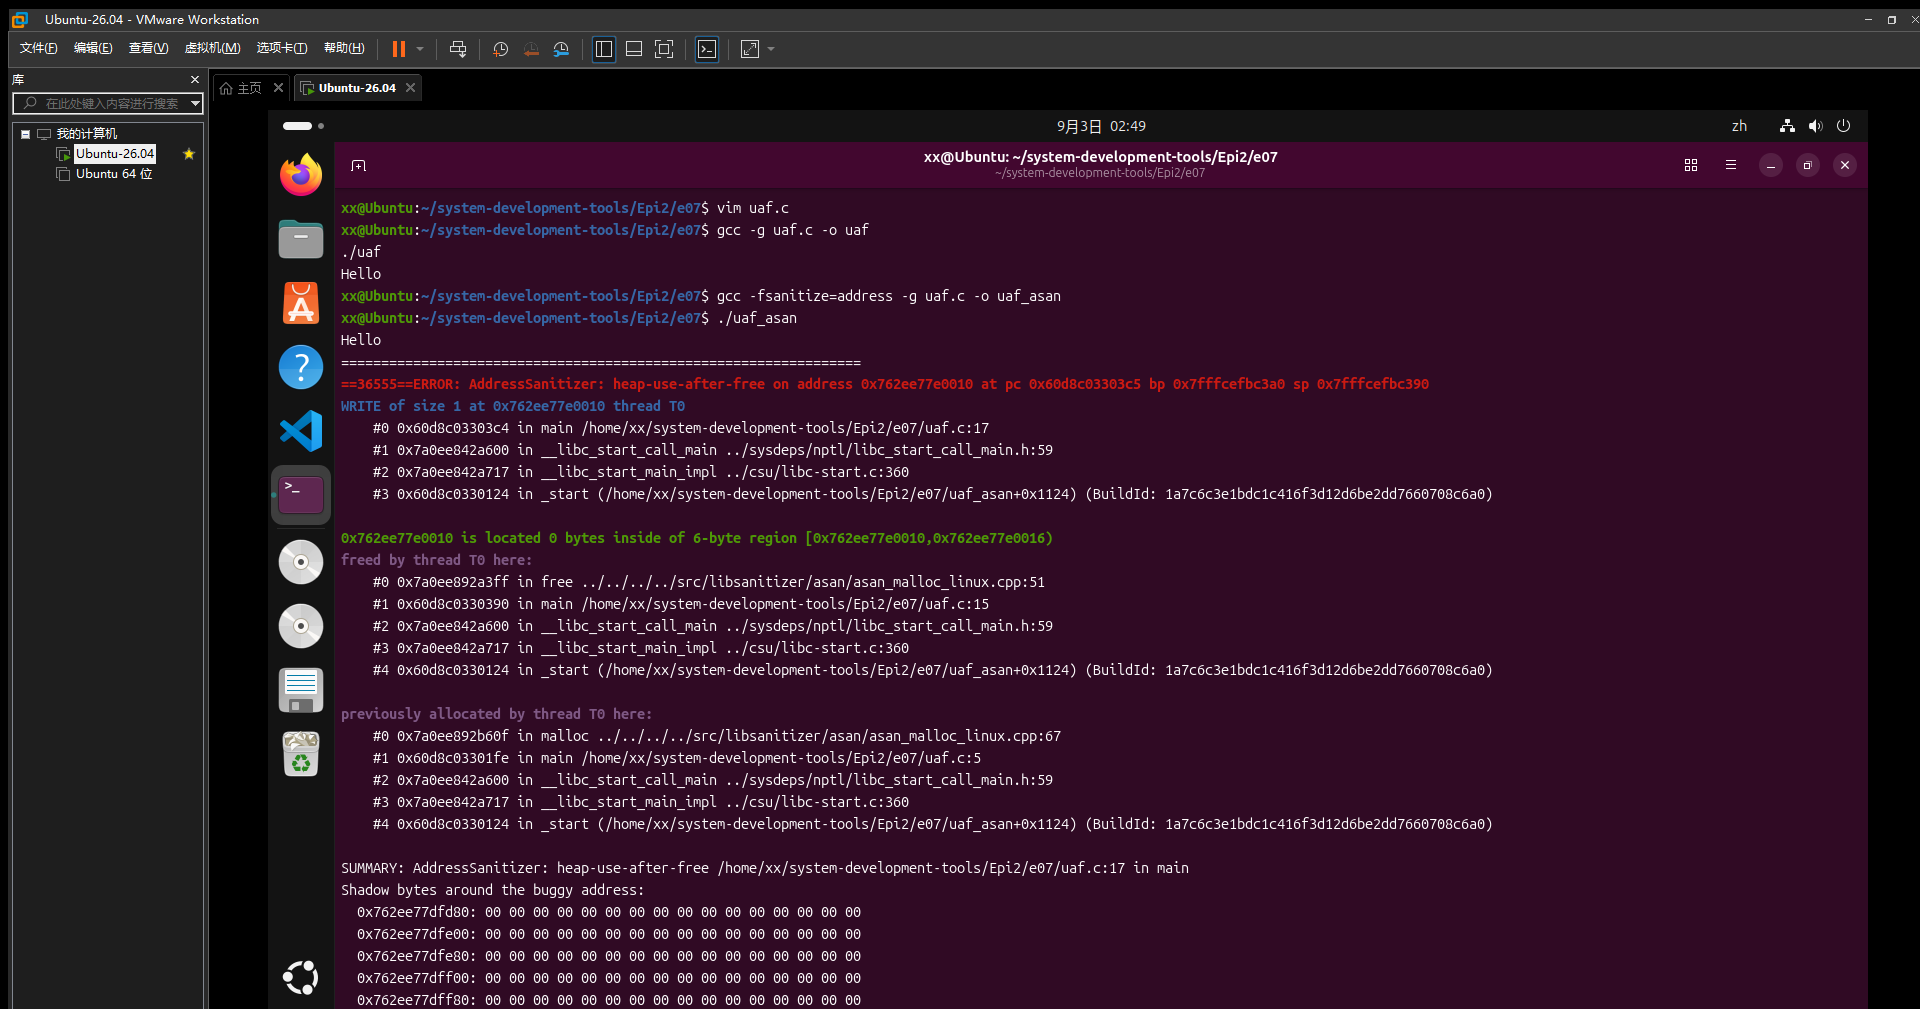
\includegraphics[width=6.65694in,height=3.95556in]{media/media/e07_1.png}

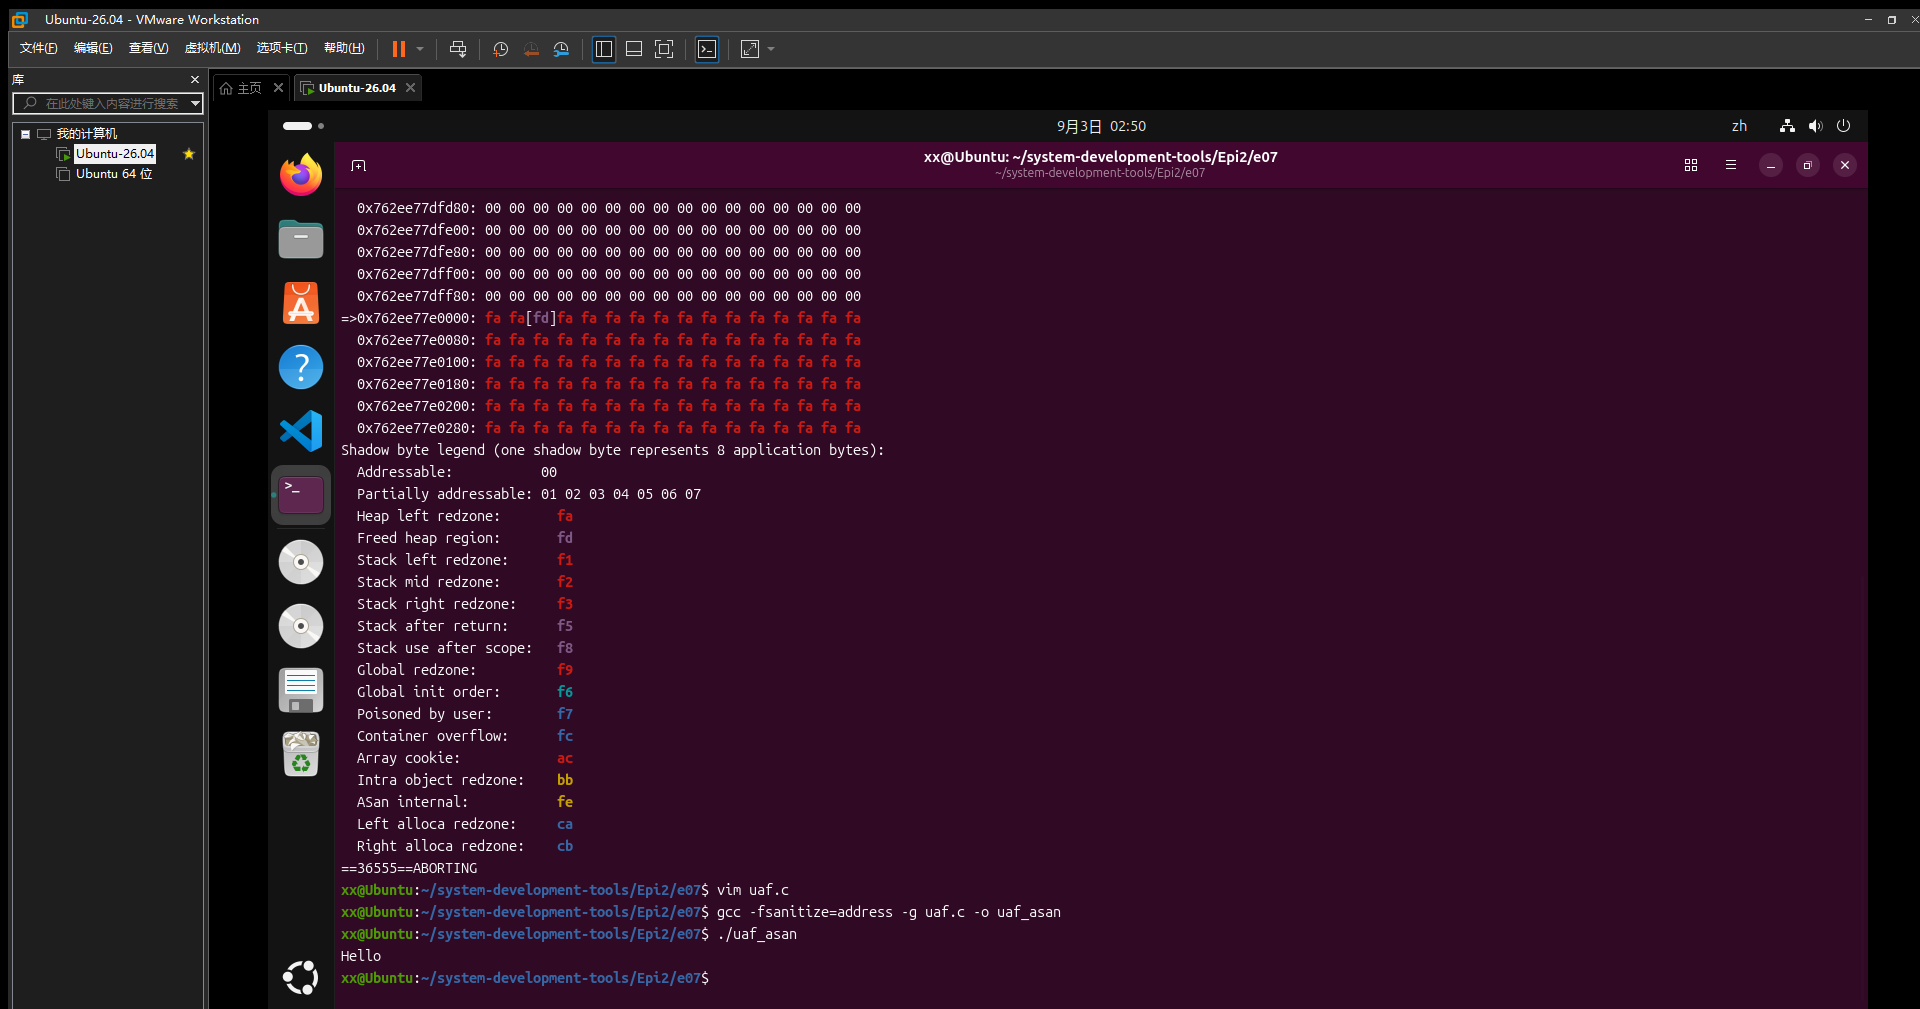
\includegraphics[width=6.65694in,height=3.95556in]{media/media/e07_2.png}

\vspace{0.6em}
\textbf{五、解题感悟}

1. 这次学会了使用 -fsanitize=address 检查内存错误。

2. AddressSanitizer 可以直接指出发生错误的代码位置。

3. 通过这次练习发现，释放内存后继续使用指针会导致严重的问题。

\vspace{1em}
\textbf{练习8：使用 strace 跟踪系统调用}

\vspace{0.6em}
\textbf{一、主题}

调试与性能分析

\vspace{0.6em}
\textbf{二、题目要求}

使用 strace 跟踪 ls -l 命令，观察程序执行过程中调用了哪些系统调用。重点关注与文件操作相关的系统调用，并分析这些系统调用的作用。

\vspace{0.6em}
\textbf{三、源程序代码}

strace ls -l

strace -e trace=file ls -l

strace -e trace=file ls -l 2\textgreater{} strace.txt

cat strace.txt

\vspace{0.6em}
\textbf{四、程序运行结果}

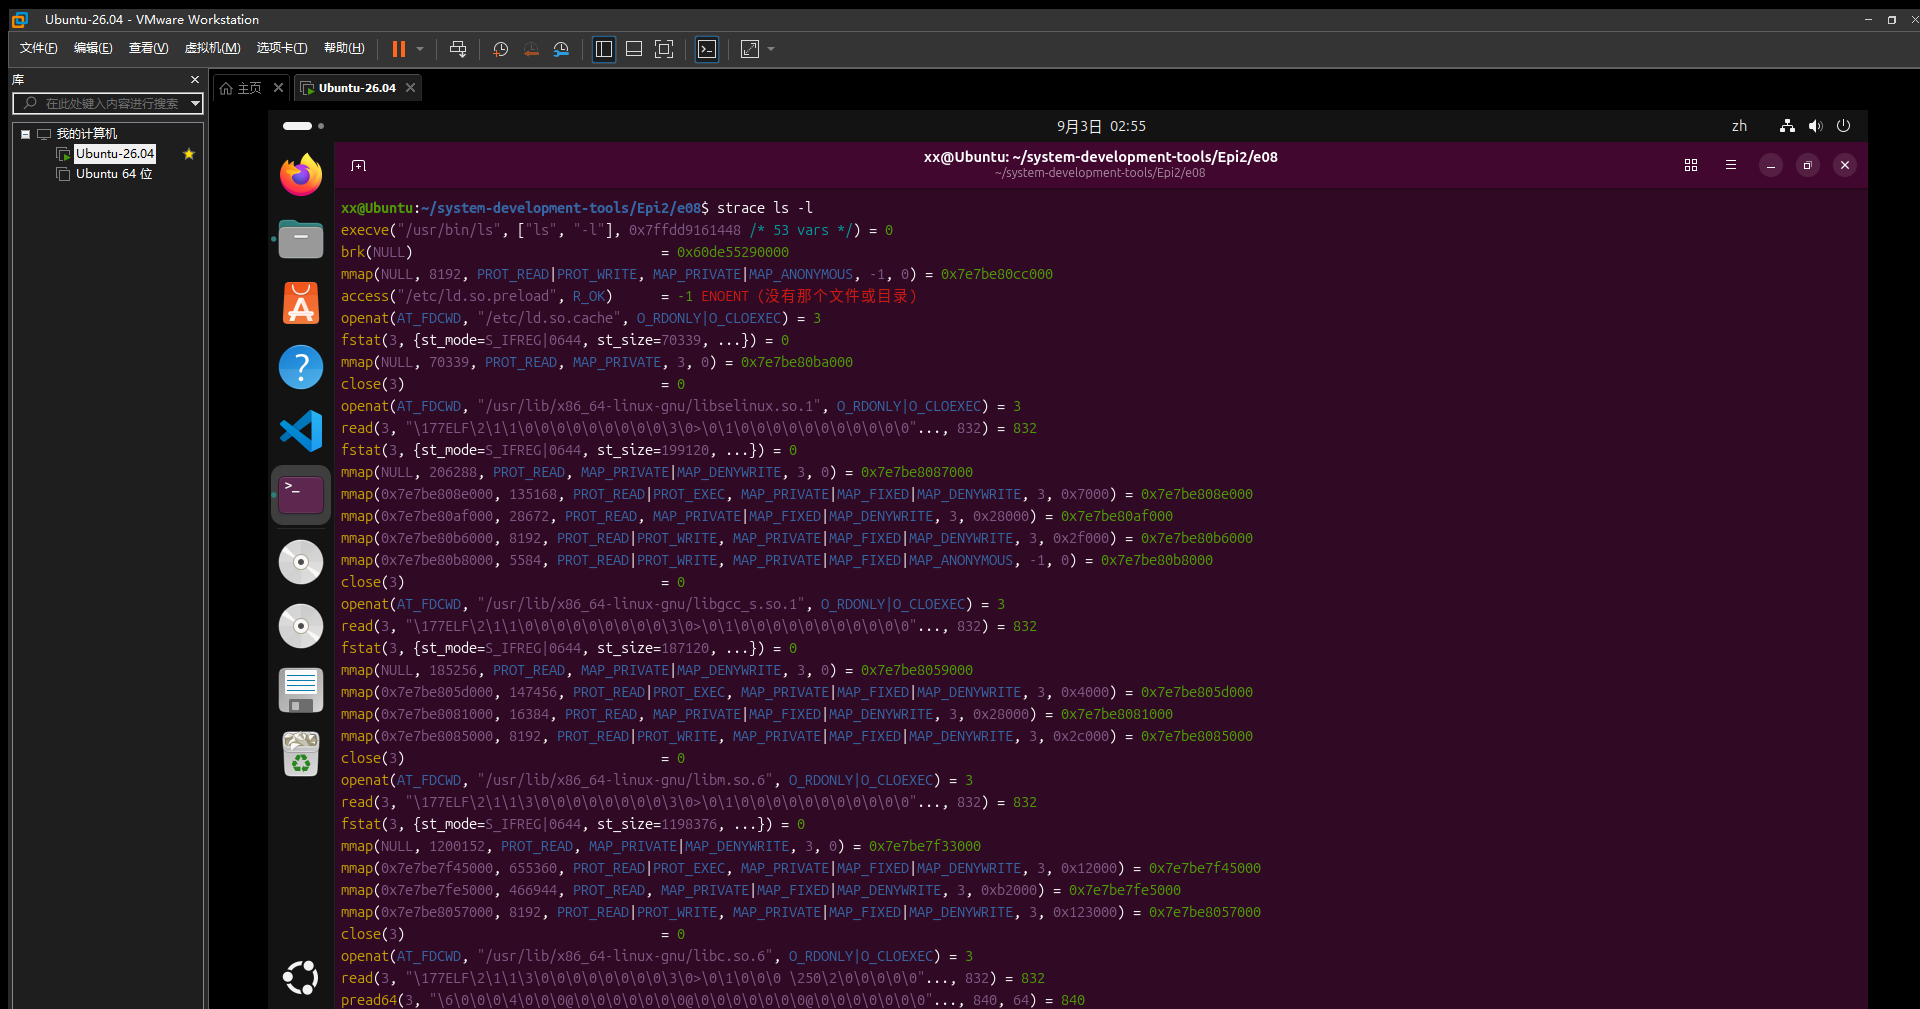
\includegraphics[width=6.65694in,height=3.95556in]{media/media/e08_1.png}

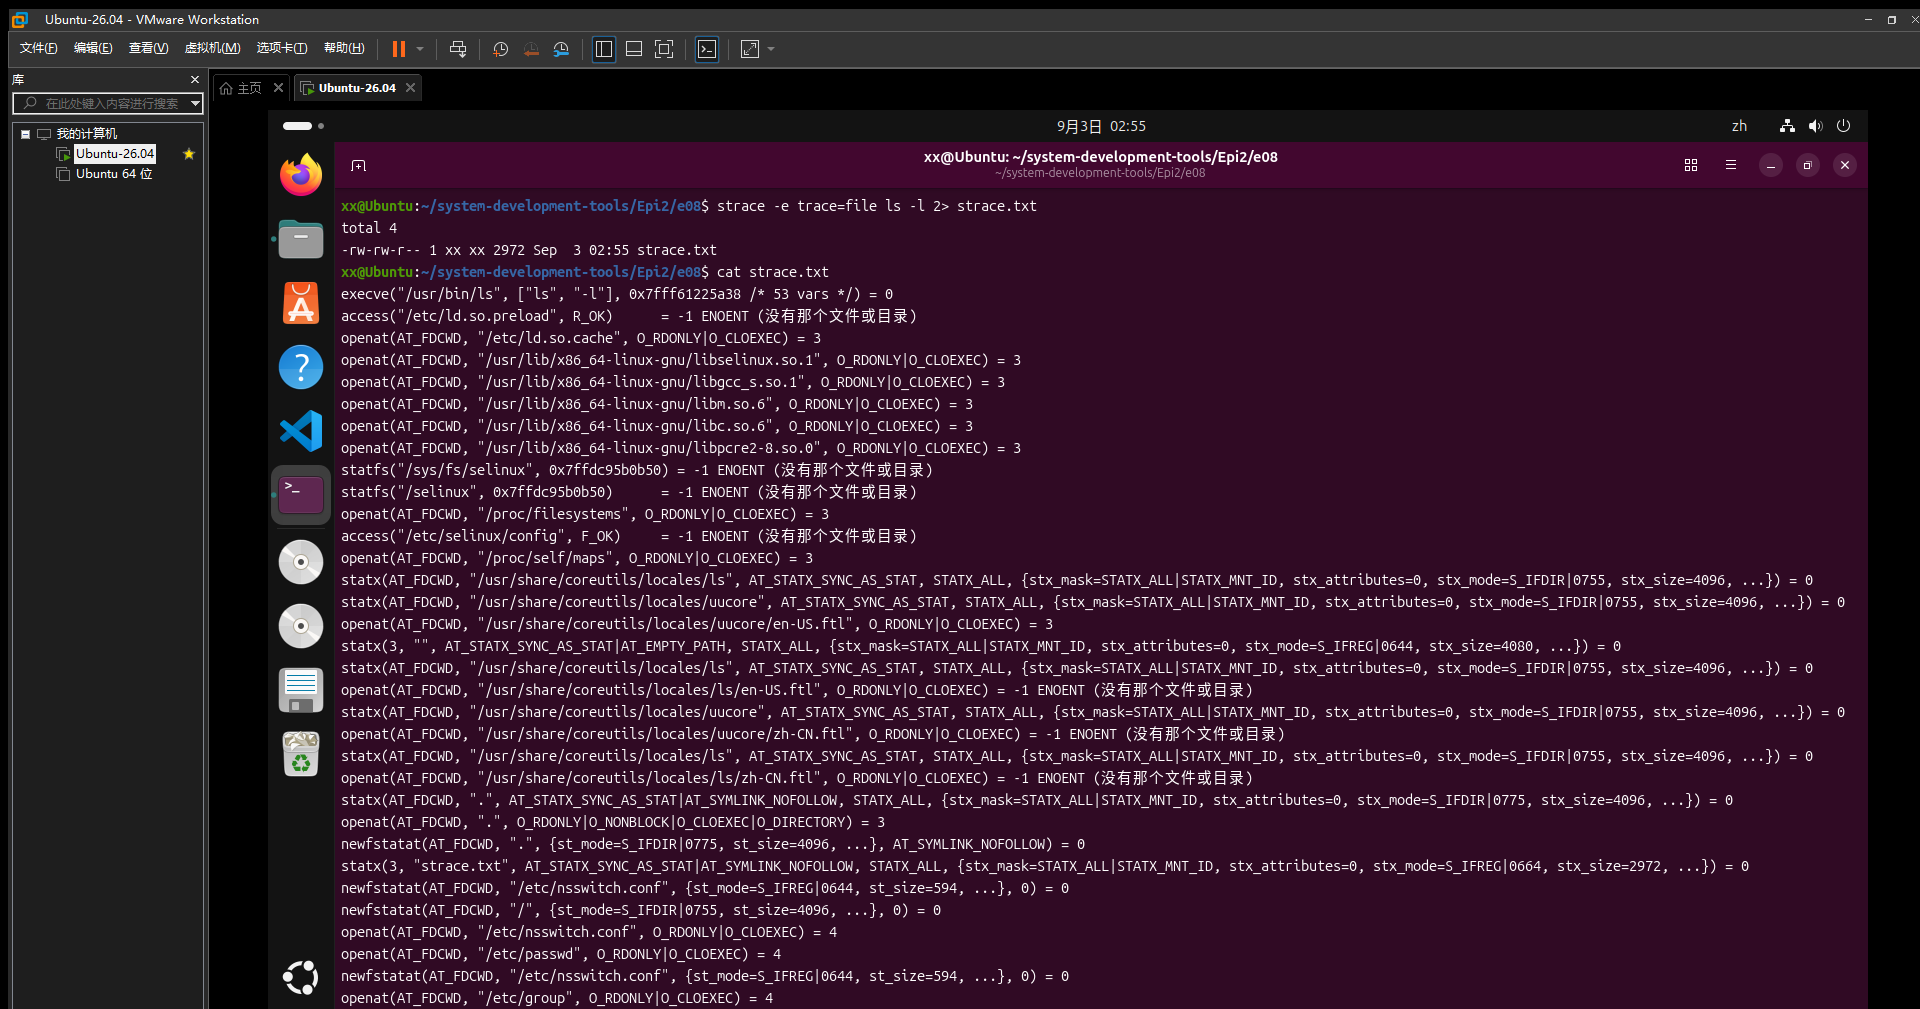
\includegraphics[width=6.65694in,height=3.95556in]{media/media/e08_2.png}

\vspace{0.6em}
\textbf{五、解题感悟}

1. 这次第一次使用 strace 查看程序的系统调用。

2. 发现一个简单的 ls 命令实际上会调用很多系统调用。

3. strace 可以帮助定位程序与操作系统之间的交互过程。

\vspace{1em}
\textbf{练习9：使用大语言模型辅助调试}

\vspace{0.6em}
\textbf{一、主题}

调试与性能分析

\vspace{0.6em}
\textbf{二、题目要求}

使用一个大语言模型（LLM）帮助调试一个难以理解的错误信息。可以尝试复制一条编译器错误信息（尤其是来自 C++ 模板或 Rust 的错误），并询问大语言模型如何解释和修复该错误。也可以尝试将 strace 或 AddressSanitizer 输出的一部分提供给大语言模型进行分析。

\vspace{0.6em}
\textbf{三、源程序代码}

无

\vspace{0.6em}
\textbf{四、程序运行结果}

llm对话：

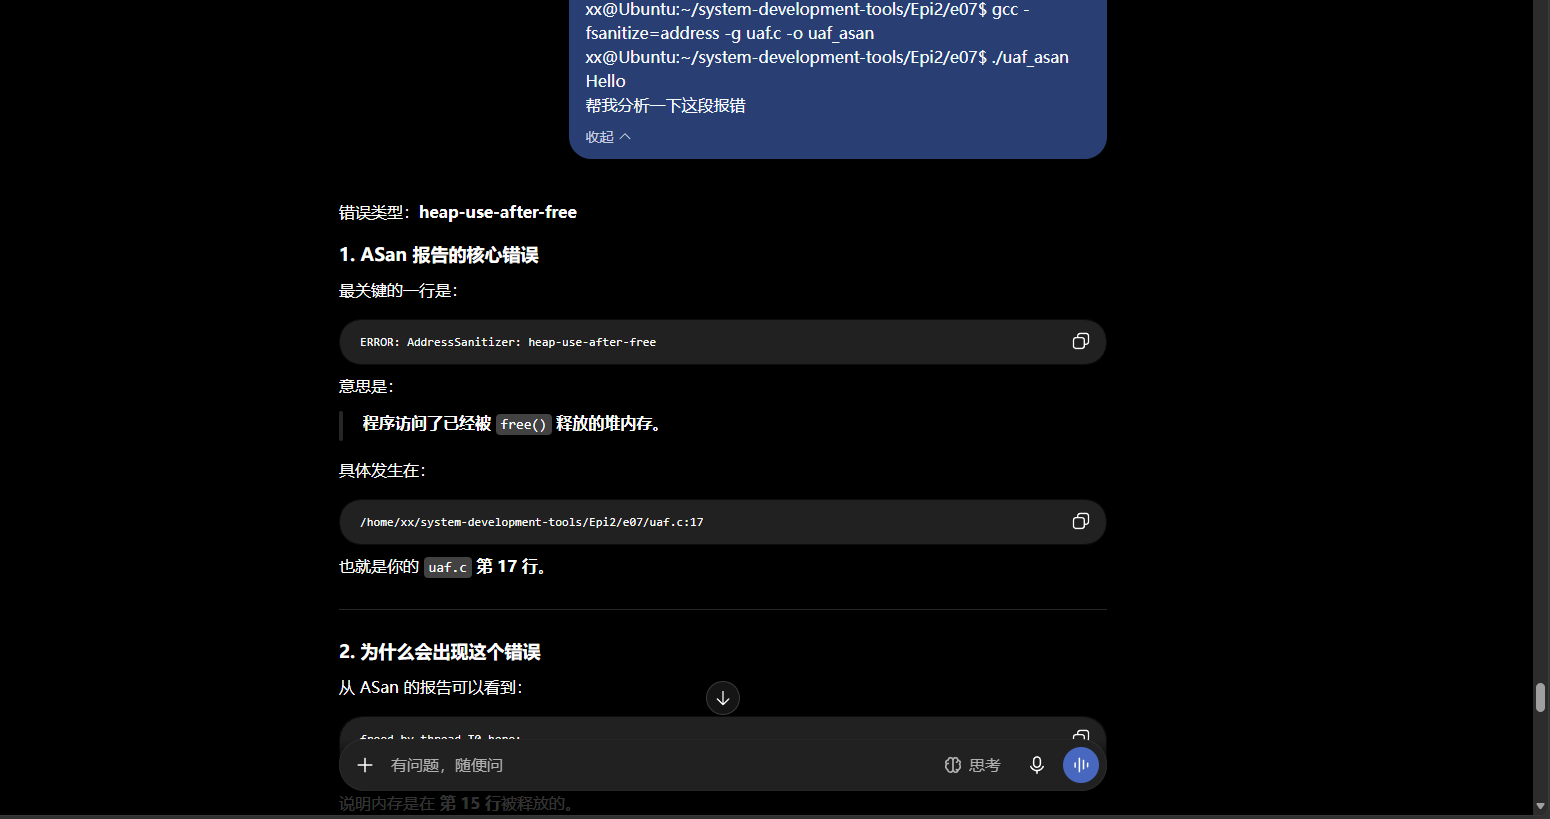
\includegraphics[width=6.65694in,height=3.95556in]{media/media/e09_1.png}

\vspace{0.6em}
\textbf{五、解题感悟}

1. 这次尝试使用大语言模型分析程序中的错误信息。

2. LLM 可以帮助快速理解复杂的报错信息并定位问题。

3. 但还是需要自己理解代码并验证修改是否正确。

\vspace{1em}
\textbf{练习10：使用 perf stat 获取性能统计信息}

\vspace{0.6em}
\textbf{一、主题}

调试与性能分析

\vspace{0.6em}
\textbf{二、题目要求}

使用 perf stat 获取一个程序的基本性能统计信息，并说明不同计数器的含义。

\vspace{0.6em}
\textbf{三、源程序代码}

vim test.c

gcc -O2 -g test.c -o test

perf stat ./test

\vspace{0.6em}
\textbf{四、程序运行结果}

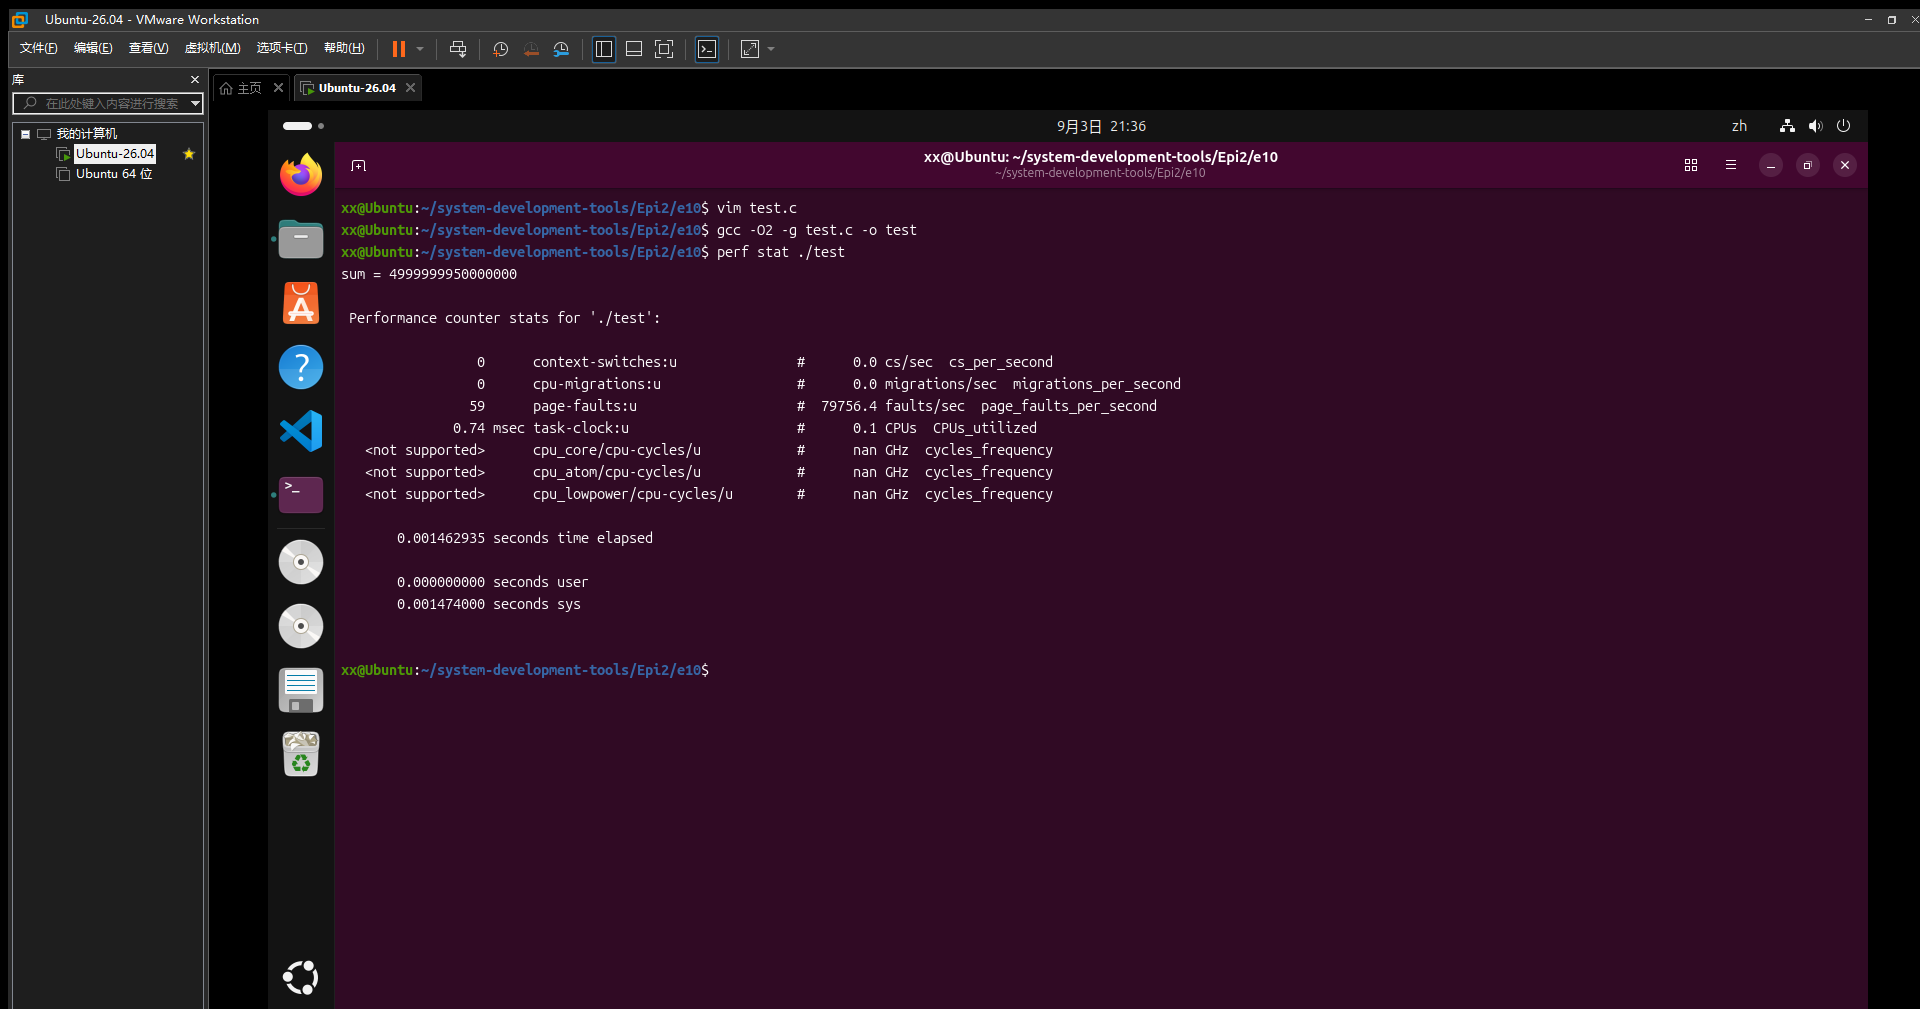
\includegraphics[width=6.65694in,height=3.95556in]{media/media/e10_1.png}

\vspace{0.6em}
\textbf{五、解题感悟}

1. 这次学习了使用 perf stat 查看程序的性能数据。

2. 了解了上下文切换、CPU 迁移和缺页异常等计数器的含义。

3. 通过这次实验发现，虚拟机环境可能不支持部分 CPU 硬件性能计数器。

\vspace{1em}
\textbf{练习11：使用 hyperfine 进行性能测试}

\vspace{0.6em}
\textbf{一、主题}

调试与性能分析

\vspace{0.6em}
\textbf{二、题目要求}

使用 hyperfine 对一个程序进行性能测试，观察程序的运行时间，并根据测试结果分析程序的性能。

\vspace{0.6em}
\textbf{三、源程序代码}

vim test.sh

chmod +x test.sh

./test.sh

hyperfine \textquotesingle{}./test.sh\textquotesingle{}

\vspace{0.6em}
\textbf{四、程序运行结果}

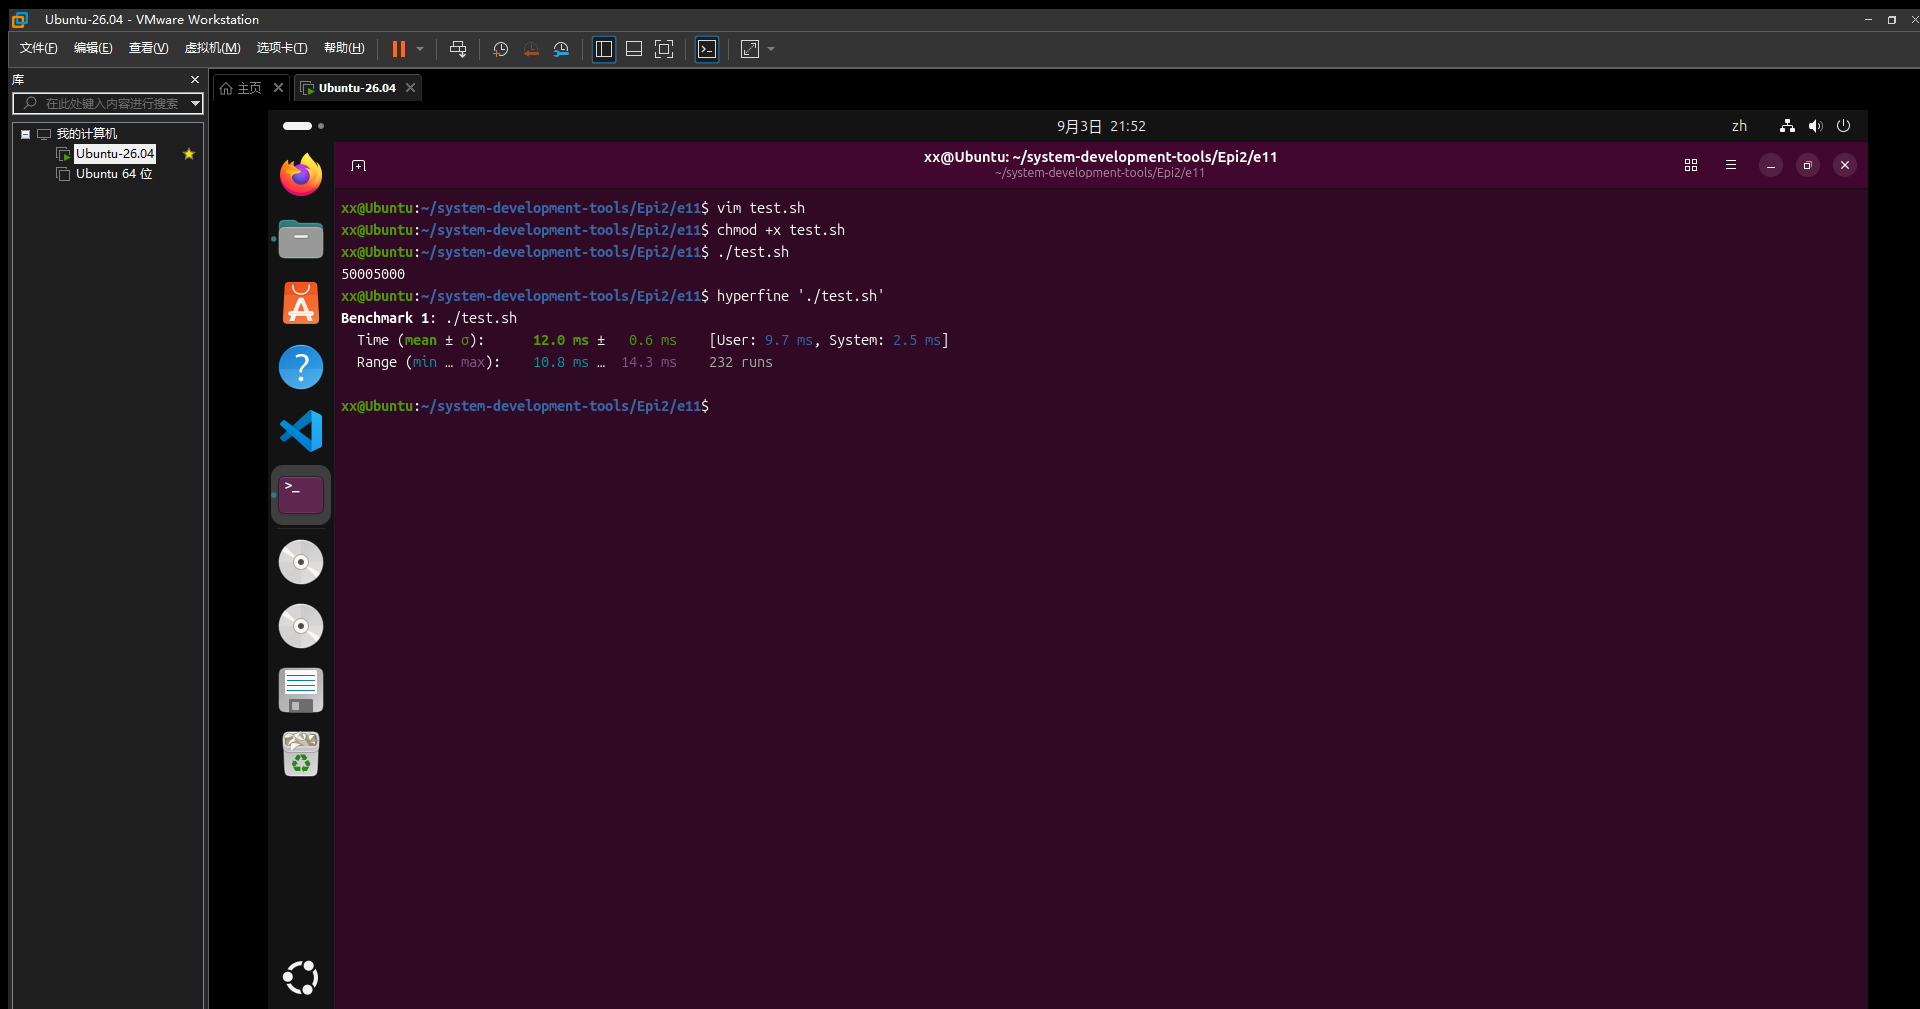
\includegraphics[width=6.65694in,height=3.95556in]{media/media/e11_1.png}

\vspace{0.6em}
\textbf{五、解题感悟}

1. 这次学习了使用 hyperfine 自动进行多次性能测试。

2. 通过平均时间和标准差可以了解程序运行速度和稳定性。

3. 多次运行可以减少单次运行时间波动对测试结果的影响。

\vspace{1em}
\textbf{练习12：查找占用 4444 端口的进程}

\vspace{0.6em}
\textbf{一、主题}

调试与性能分析

\vspace{0.6em}
\textbf{二、题目要求}

查找当前正在占用 4444 端口的进程，并确定是哪个程序正在监听该端口。

\vspace{0.6em}
\textbf{三、源程序代码}

sudo lsof -i :4444

\vspace{0.6em}
\textbf{四、程序运行结果}

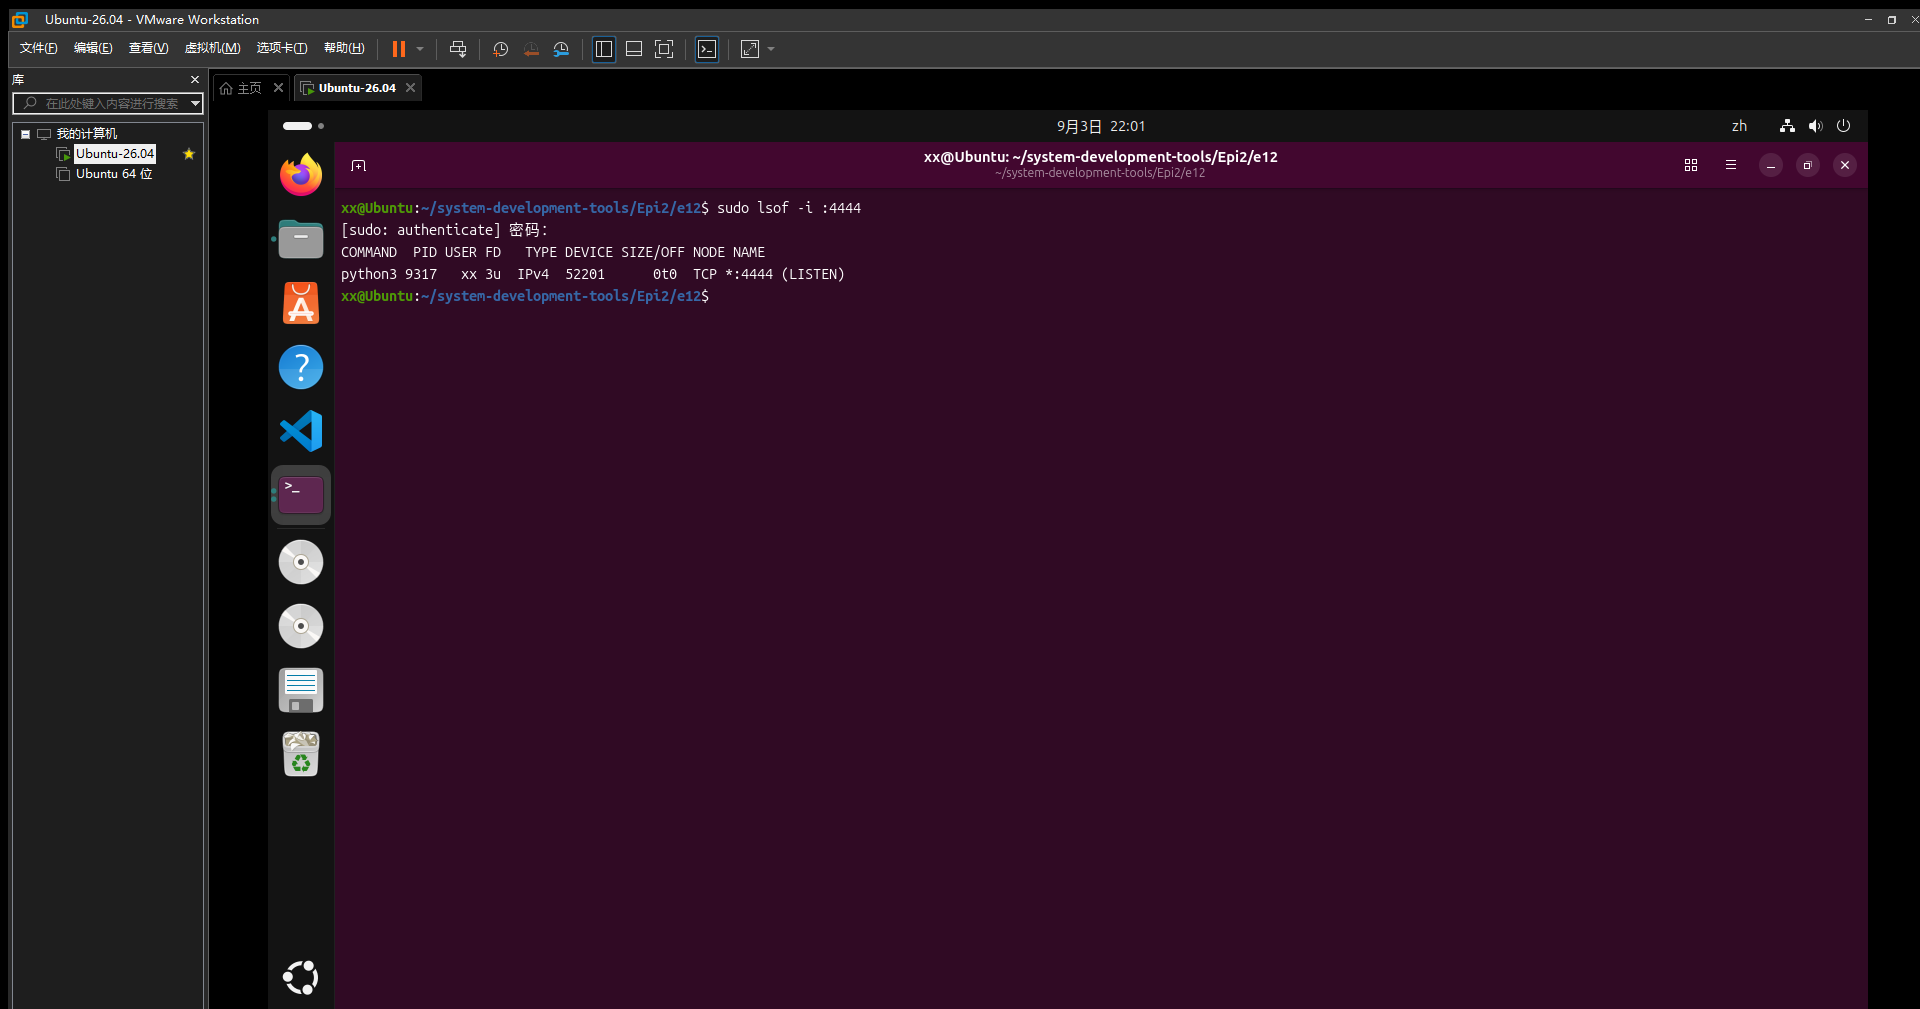
\includegraphics[width=6.65694in,height=3.95556in]{media/media/e12_1.png}

\vspace{0.6em}
\textbf{五、解题感悟}

1. 这次学习了使用 lsof 查看端口被哪个进程占用。

2. PID 可以用来确定具体的进程。

3. 通过 python3 -m http.server 4444 创建测试服务后，可以验证端口查询命令是否正常。

\end{document}
